
\begin{questions}

		\question[6] In an attempt to clean up your room, you have purchased a new floating shelf to put some of your 17 books you have stacked in a corner.  These books are all by different authors.  The new book shelf is large enough to hold 10 of the books.  Warning: before answering the next two questions, ask yourself which answer should be larger.
		\begin{parts}
			\part How many ways can you select and arrange 10 of the 17 books on the shelf?  Notice that here we will allow the books to end up in any order.  Explain.
			\begin{solution}
				We can write the answer as $P(17,10) = 17 \cdot 16 \cdot \cdots \cdot 8$, which is the same as $\frac{17!}{7!}$.  Or, if you think of picking the 10 books and then arranging those 10, you can write this as $\binom{17}{10}\cdot 10!$.  Note, that since any order is acceptable, we are distinguishing between different orders, so a permutation is appropriate here.
			\end{solution}
			\part How many ways can you arrange 10 of the 17 books on the shelf if you insist they must be arranged alphabetically by author?  Explain.
			\begin{solution}
				Here we just need to select the books, and have no choice as how to arrange them.  So the answer is just $\binom{17}{10}$
			\end{solution}
		\end{parts}





	\question[6] Consider all the functions $f: \{1,2,3,4\} \to \{1,2, 3, 4, 5, 6\}$.
		\begin{parts}
			\part How many functions are there all together?  Explain.
			\part How many functions are injective? Explain.
			\part How many of the injective functions are \emph{increasing}?  To be increasing means that if $a< b$ then $f(a) < f(b)$, or in other words, the outputs get larger as the inputs get larger. Explain.
		\end{parts}
		Hint: For all of the above, it might help to think about how you would write each function using two-line notation.
		\begin{solution}
			\begin{parts}
				\part $6^4$ functions, since for each of the 4 inputs, we have 6 choices for an output.
				\part $P(6,4) = 6 \cdot 5 \cdot 4 \cdot 3$ functions.  We have 6 choices for the image of 1, but only 5 choices for the image of 2, since we can't have repeats.  And so on, for 4 inputs.
				\part ${6 \choose 4}$.  We must select 4 different elements from the codomain to be in the range.  Once we have done this, there is only one way to assign them to inputs, since we need the outputs to be increasing.
			\end{parts}

		\end{solution}






 \question[6] Suppose you own $x$ fezzes and $y$ bow ties.  Of course, $x$ and $y$ are both greater than 1.
 \begin{parts}
 	\part How many combinations of fez and bow tie can you make?  You can wear only one fez and one bow tie at a time.  Explain.
 	\begin{solution}
 		You have $x$ choices for the fez, and for each choice of fez you have $y$ choices for the bow tie.  Thus you have $x \cdot y$ choices for fez and bow tie combination.
 	\end{solution}

 	\part Explain why the answer is {\em also} ${x+y \choose 2} - {x \choose 2} - {y \choose 2}$.  (If this is what you claimed the answer was in part (a), try it again.)
 	\begin{solution}
 		Line up all $x+y$ quirky clothing items -- the $x$ fezzes and $y$ bow ties.  Now pick 2 of them.  This can be done in ${x+y \choose 2}$ ways.  However, we might have picked 2 fezzes, which is not allowed.  There are ${x \choose 2}$ ways to pick 2 fezzes.  Similarly, the ${x+y \choose 2}$ ways to pick two items includes ${y \choose 2}$ ways to select 2 bow ties, also not allowed.  Thus the total number of ways to pick a fez and a bow ties is
 		\[{x+y \choose 2} - {x \choose 2} - {y \choose 2}\]
 	\end{solution}

 	\part Use your answers to parts (a) and (b) to give a combinatorial proof of the identity
 	\[{x+y \choose 2} - {x \choose 2} - {y \choose 2} = xy\]
 	Note: you have done almost all of the work for this problem in parts (a) and (b), now you just need to put it together into a proof.
 	\begin{solution}
 		\begin{proof}
 			The question is how many ways can you select one of $x$ fezzes and one of $y$ bow ties.  We answer this question in two ways.  First, the answer could be $a\cdot b$. This is correct as described in part (a) above.  Second, the answer could be ${x+y \choose 2} - {x \choose 2} - {y \choose 2}$.  This is correct as described in part (b) above.  Therefore
 			\[{x+y \choose 2} - {x \choose 2} - {y \choose 2} = xy\]
 		\end{proof}
 	\end{solution}

 \end{parts}




 \question[6] Consider all the triangles you can create using the points shown below as vertices.  Note, we are not allowing degenerate triangles (ones with all three vertices on the same line) but we do allow non-right triangles.

 \begin{center}
   \begin{tikzpicture}[scale=0.5]
     \foreach \i in {0,...,6} {
       \fill (\i,0) circle (2pt);
     }
     \foreach \i in {1,...,4} {
       \fill (0,\i) circle (2pt);
     }
   \end{tikzpicture}
 \end{center}

 \begin{parts}
 	\part Find the number of triangles, and explain why your answer is correct.
 	\part Find the number of triangles again, using a different method.  Explain why your new method works.
 	\part State a binomial identity that your two answers above establish (that is, give the binomial identity that your two answers a proof for).  Bonus: generalize this using $m$'s and $n$'s.
 \end{parts}

 \begin{solution}
   There are 120 triangles.  Here are a few ways (there are others as well) to get this:

   \begin{enumerate}
     \item First count the triangles with the base on the $x$-axis.  There are ${7 \choose 2}$ ways to pick the base.  The third vertex of the triangle must be one of the 4 dots on the $y$-axis (not the origin) so there are a total of ${7 \choose 2}4$ of these triangles.  The triangles with base on the $y$ axis can be counted similarly: ${5 \choose 2}6$.  However, we have counted all the right triangles twice - they have a base on the $x$-axis and also on the $y$-axis.  There are $4 \cdot 6$ right triangles.  Thus the total number of triangles is:
     \[{7 \choose 2}4 + {5 \choose 2}6 - 6\cdot 4 = 120\]
 		\item First count all the right triangles: $6 \cdot 4$.  Then count all the non-right triangles with two vertices on the $x$-axis: $4 \cdot {6 \choose 2}$.  Finally, the number of non-right triangles with two vertices on the $y$-axis: $6 \cdot {4 \choose 2}$.  All together then we have ${6 \choose 2}4 + {4 \choose 2}6 + 6 \cdot 4 = 120$.
 		\item Another approach to count the non-right triangles is to first select one of the two sides not parallel to an axis.  This can be done in $6 \cdot 4$ ways.  Then for each of these, select one of the remaining 8 points, which determines the triangle.  However, this double counts the non-right triangles, so we take $\frac{4\cdot 6 \cdot 8}{2}$, and then add on the $6\cdot 4$ right triangles.
     \item We must select 3 of the 11 dots.  This can be done in ${11 \choose 3}$ ways.  However, this will also give us degenerate triangles when all three vertices are on the $x$-axis or on the $y$-axis.  There are ${7 \choose 3}$ ways we could have picked all three vertices on the $x$-axis.  There are ${5 \choose 3}$ ways we could have picked all three vertices on the $y$-axis.  Therefore the total number of triangles is
     \[{11 \choose 3} - {7 \choose 3} - {5 \choose 3} = 120\]
   \end{enumerate}

 	Picking two of these, we know the expressions must be equal (and not just because they are equal to 120).  So we might write:
 	\[{11 \choose 3} - {7 \choose 3} - {5 \choose 3} = {7 \choose 2}4 + {5 \choose 2}6 - 6\cdot 4\]
 	In general, suppose we have $m$ dots on the $x$-axis (including the origin) and $n$ dots on the $y$-axis (including the origin).  Then counting the number of triangles in two different ways establishes:
 	\[{m+n \choose 3} - {m \choose 3} - {n \choose 3} = {m \choose 2}(n-1) + {n \choose 2}(m-1) - (m-1)(n-1)\]
 \end{solution}





 \question[6] Give a combinatorial proof of the identity:
 \[k{n\choose k} = n{n-1 \choose k-1}\]

 Hint: How many ways can you select a team of $k$ people from a group of $n$ people \emph{and} select one of them to be the team captain?
   \begin{solution}
     \begin{proof}
       Question: How many ways can you select a chaired committee of $k$ people from a group of $n$ people?  That is, you need to select $k$ people to be on the committee and one of them needs to be in charge.  How many ways can this happen?

       Answer 1: First select $k$ of the $n$ people to be on the committee.  This can be done in ${n \choose k}$ ways.  Now select one of those $k$ people to be in charge - this can be done in $k$ ways.  So there are a total of $k {n \choose k}$ ways to select the chaired committee.

       Answer 2: First select the chair of the committee.  You have $n$ people to choose from, so this can be done in $n$ ways.  Now fill the rest of the committee.  There are $n-1$ people to choose from (you cannot select the person you picked to be the chair) and $k-1$ spots to fill (the chair's spot is already taken).  So this can be done in ${n-1 \choose k-1}$ ways.  Therefore there are $n{n-1 \choose k-1}$ ways to select the chaired committee.
     \end{proof}

   \end{solution}



 	\question[6] For each of the following questions, first give one example of an outcome (i.e., on of the many things you are counting) and show how that particular outcome can be represented as a ``stars and bars'' diagram.  Then, answer the counting question.
 	\begin{parts}
 		\part When playing Yahtzee, you roll five regular 6-sided dice.  How many different outcomes are possible from a single (five dice) roll?  The order of the dice does not matter.
 		\begin{solution}
 			The outcome of (2, 3, 3, 4, 6) is represented by the diagram $|*|**|*||*$.  Each star represents a particular number that is rolled, so there should be 5 stars (since there are 5 dice).  Each bar switches from one number to the next, so there should be 5 bars.

 			Since we are counting these diagrams, the total number of outcomes is ${10 \choose 5}$.
 		\end{solution}


 		\part Your friend has 7 coins in her pocket (each could be a penny, nickel, dime or quarter).  How many different pocketfuls are possible?
 		\begin{solution}
 			One outcome is (p, p, p, n, d,d,d).  This is represented by $***|*|***|$.  Each star represents a coin.  Where that star is represents what kind of coin it is.  We need 7 stars, and 3 bars (to switch between types of coins).

 			Thus the total number of pocketfuls is ${10 \choose 7}$.
 		\end{solution}

 	\end{parts}






\end{questions}





\begin{questions}



 \question[6] Suppose you own $x$ fezzes and $y$ bow ties.  Of course, $x$ and $y$ are both greater than 1.
 \begin{parts}
 	\part How many combinations of fez and bow tie can you make?  You can wear only one fez and one bow tie at a time.  Explain.
 	\begin{solution}
 		You have $x$ choices for the fez, and for each choice of fez you have $y$ choices for the bow tie.  Thus you have $x \cdot y$ choices for fez and bow tie combination.
 	\end{solution}

 	\part Explain why the answer is {\em also} ${x+y \choose 2} - {x \choose 2} - {y \choose 2}$.  (If this is what you claimed the answer was in part (a), try it again.)
 	\begin{solution}
 		Line up all $x+y$ quirky clothing items -- the $x$ fezzes and $y$ bow ties.  Now pick 2 of them.  This can be done in ${x+y \choose 2}$ ways.  However, we might have picked 2 fezzes, which is not allowed.  There are ${x \choose 2}$ ways to pick 2 fezzes.  Similarly, the ${x+y \choose 2}$ ways to pick two items includes ${y \choose 2}$ ways to select 2 bow ties, also not allowed.  Thus the total number of ways to pick a fez and a bow ties is
 		\[{x+y \choose 2} - {x \choose 2} - {y \choose 2}\]
 	\end{solution}

 	\part Use your answers to parts (a) and (b) to give a combinatorial proof of the identity
 	\[{x+y \choose 2} - {x \choose 2} - {y \choose 2} = xy\]
 	Note: you have done almost all of the work for this problem in parts (a) and (b), now you just need to put it together into a proof.
 	\begin{solution}
 		\begin{proof}
 			The question is how many ways can you select one of $x$ fezzes and one of $y$ bow ties.  We answer this question in two ways.  First, the answer could be $a\cdot b$. This is correct as described in part (a) above.  Second, the answer could be ${x+y \choose 2} - {x \choose 2} - {y \choose 2}$.  This is correct as described in part (b) above.  Therefore
 			\[{x+y \choose 2} - {x \choose 2} - {y \choose 2} = xy\]
 		\end{proof}
 	\end{solution}

 \end{parts}




 \question[6] Consider all the triangles you can create using the points shown below as vertices.  Note, we are not allowing degenerate triangles (ones with all three vertices on the same line) but we do allow non-right triangles.

 \begin{center}
   \begin{tikzpicture}[scale=0.5]
     \foreach \i in {0,...,6} {
       \fill (\i,0) circle (2pt);
     }
     \foreach \i in {1,...,4} {
       \fill (0,\i) circle (2pt);
     }
   \end{tikzpicture}
 \end{center}

 \begin{parts}
 	\part Find the number of triangles, and explain why your answer is correct.
 	\part Find the number of triangles again, using a different method.  Explain why your new method works.
 	\part State a binomial identity that your two answers above establish (that is, give the binomial identity that your two answers a proof for).  Bonus: generalize this using $m$'s and $n$'s.
 \end{parts}

 \begin{solution}
   There are 120 triangles.  Here are a few ways (there are others as well) to get this:

   \begin{enumerate}
     \item First count the triangles with the base on the $x$-axis.  There are ${7 \choose 2}$ ways to pick the base.  The third vertex of the triangle must be one of the 4 dots on the $y$-axis (not the origin) so there are a total of ${7 \choose 2}4$ of these triangles.  The triangles with base on the $y$ axis can be counted similarly: ${5 \choose 2}6$.  However, we have counted all the right triangles twice - they have a base on the $x$-axis and also on the $y$-axis.  There are $4 \cdot 6$ right triangles.  Thus the total number of triangles is:
     \[{7 \choose 2}4 + {5 \choose 2}6 - 6\cdot 4 = 120\]
 		\item First count all the right triangles: $6 \cdot 4$.  Then count all the non-right triangles with two vertices on the $x$-axis: $4 \cdot {6 \choose 2}$.  Finally, the number of non-right triangles with two vertices on the $y$-axis: $6 \cdot {4 \choose 2}$.  All together then we have ${6 \choose 2}4 + {4 \choose 2}6 + 6 \cdot 4 = 120$.
 		\item Another approach to count the non-right triangles is to first select one of the two sides not parallel to an axis.  This can be done in $6 \cdot 4$ ways.  Then for each of these, select one of the remaining 8 points, which determines the triangle.  However, this double counts the non-right triangles, so we take $\frac{4\cdot 6 \cdot 8}{2}$, and then add on the $6\cdot 4$ right triangles.
     \item We must select 3 of the 11 dots.  This can be done in ${11 \choose 3}$ ways.  However, this will also give us degenerate triangles when all three vertices are on the $x$-axis or on the $y$-axis.  There are ${7 \choose 3}$ ways we could have picked all three vertices on the $x$-axis.  There are ${5 \choose 3}$ ways we could have picked all three vertices on the $y$-axis.  Therefore the total number of triangles is
     \[{11 \choose 3} - {7 \choose 3} - {5 \choose 3} = 120\]
   \end{enumerate}

 	Picking two of these, we know the expressions must be equal (and not just because they are equal to 120).  So we might write:
 	\[{11 \choose 3} - {7 \choose 3} - {5 \choose 3} = {7 \choose 2}4 + {5 \choose 2}6 - 6\cdot 4\]
 	In general, suppose we have $m$ dots on the $x$-axis (including the origin) and $n$ dots on the $y$-axis (including the origin).  Then counting the number of triangles in two different ways establishes:
 	\[{m+n-1 \choose 3} - {m \choose 3} - {n \choose 3} = {m \choose 2}(n-1) + {n \choose 2}(m-1) - (m-1)(n-1)\]
 \end{solution}





 \question[6] Give a combinatorial proof of the identity:
 \[k{n\choose k} = n{n-1 \choose k-1}\]

 Hint: How many ways can you select a team of $k$ people from a group of $n$ people \emph{and} select one of them to be the team captain?  Also note: $k = \binom{k}{1}$ and $n = \binom{n}{1}$, if that helps.
   \begin{solution}
     \begin{proof}
       Question: How many ways can you select a chaired committee of $k$ people from a group of $n$ people?  That is, you need to select $k$ people to be on the committee and one of them needs to be in charge.  How many ways can this happen?

       Answer 1: First select $k$ of the $n$ people to be on the committee.  This can be done in ${n \choose k}$ ways.  Now select one of those $k$ people to be in charge - this can be done in $k$ ways.  So there are a total of $k {n \choose k}$ ways to select the chaired committee.

       Answer 2: First select the chair of the committee.  You have $n$ people to choose from, so this can be done in $n$ ways.  Now fill the rest of the committee.  There are $n-1$ people to choose from (you cannot select the person you picked to be the chair) and $k-1$ spots to fill (the chair's spot is already taken).  So this can be done in ${n-1 \choose k-1}$ ways.  Therefore there are $n{n-1 \choose k-1}$ ways to select the chaired committee.
     \end{proof}

   \end{solution}



 	\question[6] For each of the following questions, first give one example of an outcome (i.e., one of the many things you are counting) and show how that particular outcome can be represented as a ``stars and bars'' diagram.  Then, answer the counting question.
 	\begin{parts}
 		\part When playing Yahtzee, you roll five regular 6-sided dice.  How many different outcomes are possible from a single (five dice) roll?  The order of the dice does not matter.
 		\begin{solution}
 			The outcome of (2, 3, 3, 4, 6) is represented by the diagram $|*|**|*||*$.  Each star represents a particular number that is rolled, so there should be 5 stars (since there are 5 dice).  Each bar switches from one number to the next, so there should be 5 bars.

 			Since we are counting these diagrams, the total number of outcomes is ${10 \choose 5}$.
 		\end{solution}


 		\part Your friend has 7 coins in her pocket (each could be a penny, nickel, dime or quarter).  How many different pocketfuls are possible?
 		\begin{solution}
 			One outcome is (p, p, p, n, d,d,d).  This is represented by $***|*|***|$.  Each star represents a coin.  Where that star is represents what kind of coin it is.  We need 7 stars, and 3 bars (to switch between types of coins).

 			Thus the total number of pocketfuls is ${10 \choose 7}$.
 		\end{solution}

 	\end{parts}


  \question[6] Consider the counting question: how many ways can you give $k$ kids $n$ identical pieces of candy, so that each kid gets at least one piece of candy?  (You might want to try some specific examples of $n$ and $k$ first, but your final answers should be done in the general case).
  \begin{parts}
    \part One way to answer this: give each kid a piece of candy first, then distribute the remaining candy without any restrictions.  How many ways can this be done?  Give your answer and describe the stars-and-bars diagrams you are counting.
    \begin{solution}
      If you give away $k$ candies, then you will have $n-k$ left, so we can use $n-k$ stars and $k-1$ bars.  The number of such diagrams is is $\binom{n-k+k-1}{k-1} = \binom{n-1}{k-1}$.
    \end{solution}
    \part Another approach: You have $n$ stars, but now can only put one bar between any two stars (and none on the ends).  How many ways can this be done?  Explain why your answer makes sense.
    \begin{solution}
      Now we have $n-1$ spots (between the stars).  Some of these get one of the $k-1$ bars, some do not.  We simply must choose which spots to put bars in.  This can be done in $\binom{n-1}{k-1}$ ways.
    \end{solution}
  \end{parts}




\end{questions}


\begin{questions}
\question[6] Write out the first 5 terms (starting with $a_0$) of each of the sequences described below.  Then give either a closed formula or a recursive definition for the sequence (whichever is NOT given in the problem).
\begin{parts}
\part $a_n = \frac{1}{2}(n^2 + n)$.
\begin{solution}
$a_0 = 0$, $a_1 = 1$, $a_2 = 3$, $a_3 = 6$ $a_4 = 10$. The sequence was described by a closed formula.  These are the triangular numbers.  A recursive definition is: $a_n = a_{n-1} + n$ with $a_0 = 0$.
\end{solution}

\part $a_n = 2a_{n-1} - a_{n-2}$ with $a_0 = 0$ and $a_1 = 1$.
\begin{solution}
This is a recursive definition.  We continue $a_2 = 2$, $a_3 = 3$, $a_4 = 4$, $a_5 = 5$, and so on.  A closed formula is $a_n = n$.
\end{solution}

\part $a_n = na_{n-1}$ with $a_0 = 1$.
\begin{solution}
We have $a_0 = 1$, $a_1 = 1$, $a_2 = 2$, $a_3 = 6$, $a_4 = 24$, $a_5 = 120$, and so on.  The closed formula is $a_n = n!$.
\end{solution}
\end{parts}

\question[8] For each sequence given below, find a closed formula for $a_n$, the $n$th term of the sequence (assume the first terms are $a_0$) by relating it to another sequence for which you already know the formula.  In each case, briefly say how you got your answers.
\begin{parts}
	\part 4, 5, 7, 11, 19, 35, \ldots
	\begin{solution}
		If we subtract 3 from each term, we get $1, 2, 4, 8, 16, 32, \ldots$, which are the powers of 2.  So we must shift this sequence up by 3 to get our sequence.  Thus
		\[a_n = 2^n + 3\]
	\end{solution}

	\part 0, 3, 8, 15, 24, 35, \ldots
	\begin{solution}
		Add 1 to each term - we get $1, 4, 9, 16, 25, 36, \ldots$, the square numbers.  So maybe our sequence as formula $a_n = n^2 - 1$.  Does this work?  $a_3 = 8$.  That is a term of our sequence, but it should be $a_2$.  So we want
		\[a_n = (n+1)^2 - 1\]
	\end{solution}

	\part 6, 12, 20, 30, 42, \ldots
	\begin{solution}
		Each term is even, so let's see what happens when we divide by 2: we get $3, 6, 10, 15, 21,\ldots$.  These are the triangle numbers, but starting at $T_2$.  We know $T_n = \frac{n(n+1)}{2}$. We want $a_0 = 2T_2$, $a_1 = 2T_3$, and so on.  In general, $a_n = 2T_{n+2}$, so
		\[a_n = (n+2)(n+3)\]
		(This is like a shift by 2 units to the left and a stretch by a factor of 2.)
	\end{solution}

	\part 0, 2, 7, 15, 26, 40, 57, \ldots (Hint: this is the \emph{sum} of two well known sequences.)
	\begin{solution}
		How far off from triangular number are these?  The triangular numbers (starting with $T_0$) are $0, 1, 3, 6, 10, 15, 21, \ldots$.  The given sequence differs from this by $0, 1, 4, 9, 16, 25, 36, \ldots$ the square numbers!  Thus
		\[a_n = \frac{n(n+1)}{2} + n^2\]
	\end{solution}
\end{parts}



% This continues to confuse students.  To fix, give the third rectangle in the sequence, or at least describe it in words.  The problem is that students want to keep attaching a square on to the same side (keep adding a 5x5 square to the 5 side in the example).
\question[8] Starting with any rectangle, we can create a new, larger rectangle by attaching a square to the longer side.  For example, if we start with a $2\times 5$ rectangle, we would glue on a $5\times 5 $ square, forming a $5 \times 7$ rectangle:

\begin{center}
	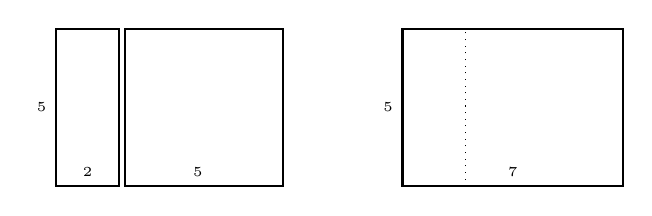
\begin{tikzpicture}[scale=.4]
		\draw[thick] (0,0) rectangle (2,5);
		\draw[thick] (2.2,0) rectangle (7.2,5);
		\draw (0,2.5) node[left]{\tiny 5} (1,0) node[above]{\tiny 2} (4.5,0) node[above]{\tiny 5};
		\draw (9,2.5) node{\Large $\rightsquigarrow$};
		\draw[thick] (11,0) rectangle (18,5);
		\draw[dotted] (13,0) -- (13,5);
		\draw (11,2.5) node[left]{\tiny 5}  (14.5,0) node[above]{\tiny 7};
	\end{tikzpicture}
\end{center}

\begin{parts}
	\part Create a sequence of rectangles using this rule starting with a $1\times 2$ rectangle.  Then write out the sequence of \emph{perimeters} for the rectangles (the first term of the sequence would be 6, since the perimeter of a $1\times 2$ rectangle is 6, the next term would be 10).
	\begin{solution}
		The rectangles are $1 \times 2$, $2 \times 3$, $3 \times 5$, $5 \times 8$, $8 \times 13$, and so on.  The sequence of perimeters is \[6, 10, 16, 26, 42, \ldots\]
	\end{solution}

	\part Repeat the above part this time starting with a $1 \times 3$ rectangle.
	\begin{solution}
		The sequence of rectangles have dimensions $1\times 3$, $3 \times 4$, $4 \times 7$, $7 \times 11$, $11\times 18$, and so on.  The sequence of perimeters is \[8, 14, 22, 36, 58, \ldots\]
	\end{solution}

	\part Find recursive definitions for each of the sequences of perimeters you found in parts (a) and (b).  Don't forget to give the initial conditions as well.
	\begin{solution}
		For the sequence from (a), the recursive formula is $a_1 = 6$, $a_2 = 10$, and $a_n = a_{n-1} + a_{n-2}$.

		For the sequence from (b), the recursive formula is $a_1 = 8$, $a_2 = 14$, and $a_n = a_{n-1} + a_{n-2}$.

		Notice that both sequence have the same rule for getting terms from the previous ones, it is just the initial conditions that are different.
	\end{solution}

	\part Are the sequences arithmetic?  Geometric?  If not, are they {\em close} to being either of these (i.e., are the differences or ratios {\em almost} constant)?  Write down the sequences of differences and sequences of ratios and explain anything interesting you find.
	\begin{solution}
		The sequences are not arithmetic because the differences between terms is not constant.  Similarly the ratio between terms is not constant, so the sequences are not geometric either.

		However, look at the ratio between terms: $10/6 \approx 1.66$, $16/10 = 1.6$, $26/16 \approx 1.625$, $42/26 \approx 1.61$, \ldots.  In fact, the ratio between terms of the second sequence also floats around this same number.

		That number (and in fact, the limit of the ratios of either sequence as the terms increase) is $\frac{1 + \sqrt{5}}{2} \approx 1.618$, also known as the golden ratio.
		\end{solution}
\end{parts}


\question[8] Consider bit strings with lenght $l$ and weight $k$ (so strings of $l$ 0's and 1's, including $k$ 1's).  We know how to count the number of these for a fixed $l$ and $k$.  Now, we will count the number of strings for which the \emph{sum} of the length and the weight is fixed.  For example, let's count all the bit strings for which $l+k = 11$.

\begin{parts}
	\part Find examples of these strings of different lengths.  What is the longest string possible?  What is the shortest?
	\begin{solution}
		The longest string is 00000000000.  If we insert a 1, we need to replace two 0's, which shortens the string.  The more 1's, the shorter the string.  We could have 111110, or 101111, or others like this (there will be 6 of them) which are shortest possible.  So all strings range in length between 6 and 11.
	\end{solution}

	\part How many strings are there of each of these lengths.  Use this to count the total number of strings (with sum 11).
	\begin{solution}
		There is 1 string with length 11.  To get a string with length 10, we need one of the 10 spots to be a 1.  Thus there are 10 of these.  To get a string of length 9, we need exactly 2 of the 9 spots to be 1's, so there are ${9 \choose 2} = 36$ such strings.  There will be ${8 \choose 3} = 56$ strings with length 8, another ${7 \choose 4} = 35$ of length 7, and finally ${6 \choose 5} = 6$ of length 6.  All together we have
		\[1 + 10 + 36 + 56 + 35 + 6 = 144 \text{ strings}\]
	\end{solution}

	\part The other approach: Let $n = l+p$ vary.  How many strings have sum $n = 1$?  How many have sum $n = 2$?  And so on.  Find and explain a recurrence relation for the sequence $(a_n)$ which gives the number of strings with sum $n$.
	\begin{solution}
		there is 1 string with sum $n = 1$ (just the string 1).  There are two strings with sum $n = 2$ (namely 11, 2).  With sum $n = 3$ we get 3 strings (111, 12, 21), and 5 with sum $n = 4$.  In fact, we recognize these as the Fibonacci numbers, which satisfy the recurrence $f_n = f_{n-1} + f_{n-2}$ with initial condition here $f_1 = 1$ and $f_2 = 2$.  The reason this is correct is that to get all the strings with sum $n$, we can start with a 1 and finish with any string with sum $n-1$, or start with a 2 and finish with any string with sum $n - 2$.  If we carry out this recurrence we find $f_{11} = 144$.
	\end{solution}


	\part Describe what you have found above in terms of Pascal's Triangle.  What patter have you discovered?
	\begin{solution}
		In this one specific case we have that \[{11\choose 0} + {10 \choose 1} + {9 \choose 2} + {8 \choose 3} + {7 \choose 4} + {6 \choose 5} = f_{11}\]
		On Pascal's triangle, we recognize that this is the sum of a diagonal line of cells (moving right, then right-up each time).  Indeed, every such sum of diagonals gives a Fibonacci number.
	\end{solution}


\end{parts}

\question[4] Bonus:  When bees play chess, they use a hexagonal board like the one shown below.  The queen bee can move one space at a time either directly to the right or angled up-right or down-right (but can never move leftwards).  How many different paths can the queen take from the top left hexagon to the bottom right hexagon?  Explain your answer, and this relates to the previous question.  (As an example, there are three paths to get to the second hexagon on the bottom row.)

	\begin{center}
	\def\r{1}
	\newcommand{\hexagon}[3]{
	  \def\x{-cos{30}*\r*#1+cos{30}*#2*\r*2}
	  \def\y{-\r*#1-sin{30}*\r*#1}
	  \draw[thick] (\x,\y) +(90:\r) -- +(30:\r) -- +(-30:\r) -- +(-90:\r) -- +(-150:\r) -- +(150:\r) -- cycle;
	  \draw (\x,\y) node{#3};
	}
	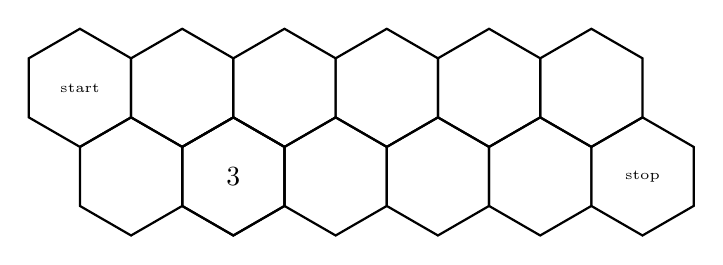
\begin{tikzpicture}[scale=.75]
	\hexagon{1}{0}{\tiny start};
	\hexagon{2}{2}{3}
	\foreach \i in {1,...,5} {
		\foreach \j in {1,2} {
			\hexagon{\j}{\i}{};
		}
	}
	\hexagon{2}{6}{\tiny stop};
	\end{tikzpicture}
	\end{center}


	\begin{solution}
		We can code each path through the hive using 0's and 1's as follows:  A 0 corresponds to a move up-right or down-right, a 1 corresponds to a move directly to the right.  Notice that a 1 move can be replaced by two consecutive 0 moves.  This describes a bijection between strings of 0's and 1's with total sum of length and weight equal to 11 and paths through the hive, so there are 144 paths.
	\end{solution}

\question[8] If you have enough toothpicks, you can make a large triangular grid.  Below, are the triangular grids of size 1 and of size 2.  The size 1 grid requires 3 toothpicks, the size 2 grid requires 9 toothpicks.

\centerline{\includegraphics[height=1in]{images/triangles.png}}

\begin{parts}
  \part Let $t_n$ be the number of toothpicks required to make a size $n$ triangular grid.  Write out the first 5 terms of the sequence $t_1, t_2, \ldots$.
  \begin{solution}
    $ 3, 9, 18, 30, 45, \ldots$
  \end{solution}

  \part Find a recursive definition for the sequence.  Explain why you are correct.
  \begin{solution}
    $t_n = t_{n-1} + 3n$ with $t_1 = 3$.  This works because to get the next larger triangular grid, we must add a row of $n$ triangles, each requiring 3 toothpicks.
  \end{solution}

  \part Is the sequence arithmetic or geometric?  If not, is it the sequence of partial sums of an arithmetic or geometric sequence?  Explain why your answer is correct.

  \begin{solution}
	  The sequence is not arithmetic (since $9-3 = 6$ but $18-9 = 9$).  It is also not geometric (since $9/3 = 3$ but $18/9 = 2$).  To decide whether the sequence is a sequence of partial sums, we look at the differences.  The sequence of differences is $6, 9, 12, 15, \ldots$.  This {\em is} an arithmetic sequence.  So we see that
	  \[t_1 = 3\]
	  \[t_2 = 3+6\]
	  \[t_3 = 3+6+9\]
	  \[t_4 = 3+6+9+12\]
	  \[t_n = \sum_{k = 1}^n 3k\]
  \end{solution}

  \part Use your results from part (c) to find a closed formula for the sequence.  Show your work.
  \begin{solution}
    We have $t_n = 3 + 6 + 9 + \cdots + 3n$.  If we reverse these and add corresponding terms we get
    \[2t_n = (3n+3) + (3n+3) + (3n+3) + \cdots + (3n+3)\]
    On the right hand side of the equation we have the sum of $n$ copies of $(3n+3)$ so we get
    \[2t_n = n(3n+3)\]
    or \[t_n = \frac{n(3n+3)}{2}\]

    This is not a huge surprise.  Notice that each term in the sequence is a multiple of 3.  Dividing each term by 3 gives the sequence $1,3, 6, 10, 15,\ldots$ - the triangular numbers. This makes sense because we are forming triangles out of 3-toothpick collections.   So a closed formula is therefore
    $t_n = 3\frac{n(n+1)}{2}$
  \end{solution}

\end{parts}


\end{questions}


\begin{questions}

\question[6] If you were to shade in a $n\times n$ square on graph paper, you could do it the boring way (with sides parallel to the edge of the paper) or the interesting way, as illustrated below:


\begin{center}
  \begin{tabular}{m{2cm}m{3cm}m{4cm}m{3cm}}
  \begin{tikzpicture}[scale=0.4]
    \draw (0,0) rectangle (1,1);
  \end{tikzpicture}
  &
  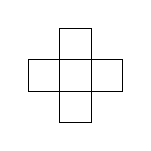
\begin{tikzpicture}[scale=0.4]
    \draw (-1,0) rectangle (2,1) (0,-1) rectangle (1,2);
  \end{tikzpicture}
  &
  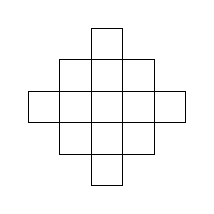
\begin{tikzpicture}[scale=0.4]
    \draw (-2,0) rectangle (3,1) (0,-2) rectangle (1,3) (-1,-1) rectangle (2,2);
  \end{tikzpicture}
  &
  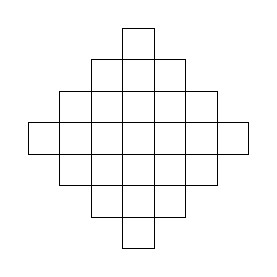
\begin{tikzpicture}[scale=0.4]
    \draw (-3,0) rectangle (4,1) (-2,-1) rectangle (3,2) (-1,-2) rectangle (2,3) (0,-3) rectangle (1,4);
  \end{tikzpicture}
\end{tabular}
\end{center}

The interesting thing here, is that a $3\times 3$ square now has area 13.  Our goal is the find a formula for the area of a $n \times n$ (diagonal) square.

\begin{parts}
  \part Write out the first few terms of the sequence of areas (assume $a_1 = 1$, $a_2 = 5$, etc).  Is the sequence arithmetic or geometric?  If not, is it the sequence of partial sums of an arithmetic or geometric sequence?  Explain why your answer is correct, referring to the diagonal squares.

  \begin{solution}
    The sequence is $1, 5, 13, 25, 41, 61, \ldots$.  This is not arithmetic
	  (since $5-1 = 4$ but $13-5 = 8$).  It is also not geometric (since $5/1 = 5$ but $13/5 = 2.6$).  To recognize whether the sequence is a sequence of partial sums, we look at the differences.  The sequence of differences is $4, 8, 12, 16, 20, \ldots$.  This {\em is} an arithmetic sequence.  So we see that
	  \[a_1 = 1\]
	  \[a_2 = 1+4\]
	  \[a_3 = 1+4+8\]
	  \[a_4 = 1+4+8+12\]
	  \[a_n = 1 + \sum_{k = 1}^n 4(k-1)\]
  \end{solution}

  \part Use your results from part (a) to find a closed formula for the sequence.  Show your work.  Note, while there are lots of ways to find a closed formula here, you should use partial sums specifically.
  \begin{solution}
    We have $a_n = 1 + 4 + 8 + \cdots + 4(n-1)$.  If we reverse these and add corresponding terms (not including the 1) we get
    \[2a_n = 2 + (4n) + (4n) + (4n) + \cdots + (4n)\]
    On the right hand side of the equation we have the sum of $n-1$ copies of $(4n)$ so we get
    \[2a_n = 2 + (n-1)(4n)\]
    or \[a_n = 2n^2 - 2n + 1\]
  \end{solution}
\end{parts}



\question[8] In their down time, ghost pirates enjoy stacking cannonballs in triangular based pyramids (aka, tetrahedrons), like those pictured here:

\centerline{

\begin{tikzpicture}
\draw (0,0) circle (10pt);
\draw[very thin, color=brown!15] (0,0) circle (10pt);
\shade[shading=axis,bottom color=black!70!brown, top color=black!15, shading angle=-40] (0,0) circle (10pt);
\end{tikzpicture}\qquad

\begin{tikzpicture}
\foreach \pos in {(-.32, .2), (.32,.2), (0,.55), (0,0)}{
\draw[very thin, color=brown!15] \pos circle (10pt);
\shade[shading=axis,bottom color=black!70!brown, top color=black!15, shading angle=-40] \pos circle (10pt);
}
\end{tikzpicture}
\qquad

\begin{tikzpicture}
\foreach \pos in {(-.64, .4), (.64,.4), (-.37, .75), (.37,.75), (0, 1.2), (-.32, .2), (.32,.2), (0,.6), (0,0)}{
\draw[very thin, color=brown!15] \pos circle (10pt);
\shade[shading=axis,bottom color=black!70!brown, top color=black!15, shading angle=-40] \pos circle (10pt);
}
\end{tikzpicture}
}

Note, these are solid tetrahedrons, so there will be some cannonballs obscured from view (the picture on the right has one cannonball in the back not shown in the picture, for example).


The pirates wonder how many cannonballs would be required to build a pyramid 15 layers high (thus breaking the world cannonball stacking record).  Can you help?  Find a closed formula for the number of cannonballs in the $n$th pyramid and use this to find the number of cannonballs in the 15th pyramid.

\begin{solution}
  To get the next larger pyramid, we add a triangle of cannonballs to the previous pyramid.  Thus to get $P_n$, we add $P_{n-1}$ to the $n$th triangular number:
  $P_3 = 4 + 6 = 10$, $P_4 = 10 + 10 = 20$, $P_5 = 20 + 15 = 35$.

  	To find the closed formula, look at the sequences of differences.  The first differences are $3, 6, 10, 15, \ldots$.  The second differences are $3, 4, 5, 6, \ldots$.  The third differences are $1,1,1,\ldots$.  Since third differences are constant, we know the closed formula for $P_n$ will be a degree 3 polynomial.  So $P_n = an^3 + b n^2 + cn + d$.  Note that $P_0 = 0$, so $d = 0$.  To solve for $a$, $b$, and $c$, we solve the system of equations:
  \begin{align*}
    1 & = a + b + c \\
    4 & = 8a+ 4b + 2c \\
    10 & = 27a + 9b + 3c
  \end{align*}
  Doing so gives $a = \frac{1}{6}$, $b = \frac{1}{2}$ and $c = \frac{1}{3}$ so
  \[P_n = \frac{1}{6}n^3 + \frac{1}{2} n^2 + \frac{1}{3} n\]

Finally:
  \[P_{15} = \frac{1}{6}15^3 + \frac{1}{2} 15^2 + \frac{1}{3} 15 = 680\]
\end{solution}




\question Let $a_n$ be the number of  $1 \times n$ tile designs can you make using $1 \times 1$ squares available in 4 colors and $1 \times 2$ dominoes available in 5 colors.
\begin{parts}
	\part[3] First, find a recurrence relation to describe the problem.  Explain why the recurrence relation is correct (your explanation should reference tile designs of squares and dominoes).
	\begin{solution}
		$a_n = 4a_{n-1} + 5a_{n-2}$.  Each path of length $n$ must either start with one of the 4 $1\times 1$ tiles, in each case there are then $a_{n-1}$ ways to finish the path, or start with one of the 5 $1\times 2$ tiles, in each case there are then $a_{n-2}$ ways to finish the path.
	\end{solution}

	\part[2] Write out the first 6 terms of the sequence $a_1, a_2, \ldots$.  Hint: since you have a recurrence relation, the only difficult part will be finding the first two terms, which are simple counting questions.
	\begin{solution}
		4, 21, 104, 521, 2604, 13021
	\end{solution}

	\part[3] Solve the recurrence relation.  That is, find a closed formula for $a_n$.
	\begin{solution}
		The characteristic equation is $x^2 - 4x - 5 = 0$ so the characteristic roots are $x = 5$ and $x = -1$.  Therefore the general solution is
		\[a_n = a 5^n + b (-1)^n\]
		We solve for $a$ and $b$ using the fact that $a_1 = 4$ and $a_2 = 21$.  We get $a = \frac{5}{6}$ and $b = \frac{1}{6}$.  Therefore the solution is
		\[a_n = \frac{5}{6} 5^n + \frac{1}{6}(-1)^n\]
	\end{solution}

\end{parts}


\question[8] Consider the sequences $2, 5, 12, 29, 70, 169, 408,\ldots$ (with $a_0 = 2$).
\begin{parts}
\part Describe the rate of growth of this sequence.
\begin{solution}
It does not seem to help to look at the difference between terms - in fact, the differences seem to be growing in the same manner as the original sequence.  However, looking at the ratio between terms gives us almost a common ratio of 2.  In other words, it appears that the sequence is growing exponentially.
\end{solution}


\part Find a recursive definition for the sequence.
\begin{solution}
We see that $5$ is a little more than twice the previous term, and 12 is a little more than twice 5.  In fact, it is exactly 2 more, which is the first term.  So perhaps $a_n = 2a_{n-1} + a_{n-2}$, and this seems to work moving forward.
\end{solution}

\part Find a closed formula for the sequence.  Don't be afraid to use the quadratic formula.

\begin{solution}
Use the characteristic root technique.  The characteristic equation is $x^2 - 2x - 1 = 0$.  Solving this (using the quadratic formula) gives $x = 1\pm\sqrt{2}$.  So we know that the closed formula for $a_n = a(1+\sqrt{2})^n + b(1-\sqrt{2})^n$.  Now let's find $a$ and $b$.  We have

\[2 = a + b\]
\[5 = a(1+\sqrt{2}) + b(1-\sqrt{2})\]
Use substitution: $a = 2-b$ so $5 = (2-b)(1+\sqrt 2) + b(1-\sqrt{2})$ which simplifies to $b = 1-\frac{3}{2 \sqrt{2}}$.  This gives $a = 1+\frac{3}{2\sqrt 2}$.  Therefore
\[a_n = (1+\frac{3}{2\sqrt 2})(1+\sqrt{2})^n + (1-\frac{3}{2 \sqrt{2}})(1-\sqrt{2})^n\]
\end{solution}

\part If you look at the sequence of differences between terms, and then the sequence of second differences, the sequence of third differences, and so on, will you ever get a constant sequence?  Explain how you know.
\begin{solution}
You will never get a constant sequence of differences.  If you did, this would mean that the original sequence would be some polynomial.  But we have an exponential closed formula, so no polynomial will fit.
\end{solution}
\end{parts}

\question[4] Bonus: For the sequence in problem 1, find the closed formula in as many interesting ways as you can.  Each unique explanation gets 1 point.

\begin{solution}
  There are lots of interesting things you can do here.  From what we have done with sequences, you could notice that the second differences are constant, so you know that the closed formula will be quadratic.  You could then use polynomial fitting, or simply compare the sequence to $n^2$ to find the pattern.  More inventive solutions include:
  \begin{enumerate}
    \item Look along the diagonals.  The $n$th figure will have $n$ diagonals of $n$ squares, and $n-1$ diagonals of $n-1$ squares.  Thus all together, the number of squares is $n^2 + (n-1)^2$.
    \item If you count the number of squares in each row starting at the top, you will have $1, 3, 5, \ldots, 2n-3, 2n-1, 2n-3, \ldots, 3, 1$.  So we can think of the total number of squares as being the sum of the first $n$ odd numbers (counting up) plus the sum of the first $n-1$ odd numbers (counting down).  But the sum of the first $n$ odd numbers is $n^2$, so again we find the total number of squares to be $n^2 + (n-1)^2$.
    \item Enclose the figure in a larger square with dimensions $2n-1 \times 2n-1$.  Then look at what part of that square you don't want.  You have 4 triangles you must remove.  The $n$th figure requires removing a triangle with base $n-1$ on each corner, so we must remove $4T_{n-1}$, where $T_n = \frac{n(n+1)}{2}$ is the $n$th triangular number.  Thus the total number of squares in the figure is
    \[(2n-1)^2 - 4\frac{(n-1)n}{2}.\]
  \end{enumerate}
\end{solution}


\end{questions}


\question[6] On the way to the market, you exchange your cow for some magic dark chocolate espresso beans.  These beans have the property that every night at midnight, each bean splits into two, effectively doubling your collection.  You decide to take advantage of this and each morning (around 8am) you eat 5 beans.
\begin{parts}
\part Explain why it is true that \emph{if} at noon on day $n$ you have a number of beans ending in a 5, then at noon on day $n+1$ you will still have a number of beans ending in a 5.

\begin{solution}
If we have a number of beans ending in a 5 and we double it, we will get a number of beans ending in a 0 (since $5\cdot 2 = 10$).  Then if we subtract 5, we will once again get a number of beans ending in a 5.  Thus if on any day we have a number ending in a 5, the next day will also have a number ending in a 5.

\end{solution}

\part Why is the previous fact not enough to conclude that you will always have a number of beans ending in a 5? What additional fact would you need?
\begin{solution}
If you don't \emph{start} with a number of beans ending in a 5 (on day 1), the above reasoning is still correct but not helpful.  For example, if you start with a number ending in a 3, the next day you will have a number ending in a 1.
\end{solution}

\part Assuming you have the additional fact in part (b), and have successfully proved the fact in part (a), how do you know that you will always have a number of beans ending in a 5?  Illustrate what is going on by carefully explaining how the two facts above prove that you will have a number of beans ending in a 5 on \textbf{day 4} specifically.  In other words, explain why induction works in this context.
\begin{solution}
Part (b) is the base case and part (a) is the inductive case.  If on day 1 we have a number ending in a 5 (by part (b)), then on day 2 we will also have a number ending in a 5 (by part (a)).  Then by part (a) again, we will have a number ending in a 5 on day 3.  By part (a) again, this means we will have a number ending in a 5 on day 4.

The proof by induction would say that on \emph{every} day we will have a number ending in a 5, and this works because we can start with the base case, then use the inductive case over and over until we get up to our desired $n$.
\end{solution}
\end{parts}



\question[8] Find the largest number of points which a football team cannot get exactly using just 3-point field goals and 7-point touchdowns (ignore the possibilities of safeties, missed extra points, and two point conversions).  Prove your answer is correct by mathematical induction.

\begin{solution}
  First note that it is impossible to make 11 points -- if only field goals are made, the points must be a multiple of 3, if 1 touchdown is made, the possible point totals are 7, 10, 13, \ldots and two touchdowns are already too much.

  We will prove that 11 is the largest number of points which cannot be made.  In other words, any number of points greater than or equal to 12 can be made.

  \begin{proof}
    Let $P(n)$ be the statement ``it is possible to make $n$ points using touchdowns and field goals.''  We will prove $P(n)$ is true for all $n \ge 12$.

    First the base case: You can make 12 points with 4 field goals, so $P(12)$ is true.

    Now the inductive case: Assume $P(k)$ is true for some fixed $k \ge 12$.  That is, it is possible to make $k$ points.  Since $k \ge 12$, we must have made the $k$ points using either at least 2 field goals or at least 2 touchdowns, or both (because if we used just one of each we would have only 10 points).  Now if the $k$ points were accomplished with 2 (or more) field goals, then replace 2 field goals with 1 touchdown.  This increases to point total by 1, giving $k + 1$ points.  On the other hand, if the $k$ points were accomplished with $2$ (or more) touchdowns, replace 2 touchdowns with 5 field goals, again increasing the point total by 1, giving $k+1$ points.  Using one of these two substitutions, we can make $k+1$ points, so $P(k+1)$ is true, establishing the inductive case.

    Therefore by the principle of mathematical induction, $P(n)$ is true for all $n \ge 12$.
  \end{proof}
\end{solution}


\question[8] Prove, by mathematical induction, that $F_0 + F_1 + F_2 + \cdots + F_{n} = F_{n+2} - 1$, where $F_n$ is the $n$th Fibonacci number ($F_0 = 0$, $F_1 = 1$ and $F_n = F_{n-1} + F_{n-2}$).
\begin{solution}
This is saying that if we add up the first $n$ Fibonacci numbers, we will get another Fibonacci number (specifically, the $(n+2)$th one).  Induction is a good idea here because it will be easy to just add one more Fibonacci number to the sum we already have.  If we already have $F_{k+2}$ and we add $F_{k+1}$ we can use the recurrence relation to simplify this, becoming $F_{k+3}$.

  \begin{proof}
    Let $P(n)$ be the statement $F_0 + F_1 + F_2 + \cdots + F_n = F_{n+2} - 1$.  We will prove that $P(n)$ is true for all $n \ge 0$.

    Base case: $P(0)$ states that $F_0 = F_2 - 1$, which is true because $F_0 = 0$ and $F_2 = 1$.

    Inductive case:  Assume $P(k)$ is true for an arbitrary fixed $k \ge 0$.  That is, \[F_0 + F_1 + F_2 + \cdots + F_k = F_{k+2} - 1\]
    We must prove that $P(k+1)$ is true as well (i.e. that $F_0 + F_1 + \cdots +F_{k+1} = F_{k+3} - 1$).  Start with the left hand side:
    \begin{align*}
      F_0 + F_1 + F_2 + \cdots + F_k + F_{k+1} & = F_{k+2} - 1 + F_{k+1} & \mbox{ by the inductive hypothesis}\\
      & = F_{k+3} - 1 & \mbox{ by the definition of the Fibonacci numbers}
    \end{align*}
    Thus $P(k+1)$ is true.

    Therefore by the principle of mathematical induction, $P(n)$ is true for all $n \ge 0$.
  \end{proof}

\end{solution}

\question[8] Prove that the sum of the interior angles of a convex $n$-gon is $(n-2)\cdot 180^\circ$.  (A convex $n$-gon is a polygon with $n$ sides for which each interior angle is less than $180^\circ$.)  Hint: start with $(k+1)$-gon and divide it up into a $k$-gon and a triangle.

\begin{solution}
Every $n$-gon (for $n \ge 4$) can be divided into a triangle and a $(n-1)$-gon by drawing a line between two vertices one apart.  The sum of the interior angles of the $n$-gon will then be the sum of the angles in the triangle and the angles in the $(n-1)$-gon.  This shows how we can go from one case to the next.  Since we are adding a triangle, we are adding $180^\circ$ to the sum, which is what incrementing $n$ in $(n-2)\cdot 180^\circ$ does.

\begin{proof}
Let $P(n)$ be the statement, ``the sum of the interior angles of a convex $n$-gon is $(n-2)\cdot 180^\circ$.''  We will prove $P(n)$ is true for all $n \ge 3$.

Base case: When $n=3$, we have a triangle, and we know the sum of the interior angles of a triangle is $180^\circ = (3-2)\cdot 180^\circ$.  Thus $P(3)$ is true.

Inductive case: Assume $P(k)$ is true for some arbitrary $k \ge 3$.  That is, the sum of the angles of any convex $k$-gon is $(k-2)\cdot 180^\circ$.  Now consider an arbitrary convex $(k+1)$-gon.  Draw an edge between two vertices one apart (for example, between the first and third vertices counting clockwise).  Since we have at least 4 vertices, this is a new edge, and divides the $k+1$-sided polygon into a convex $k$-gon and a triangle.  The sum of the angles of the $(k+1)$-gon will be exactly the sum of the angles in the $k$-gon plus the sum of the angles of the triangle.  But the $k$-gon has sum of angles $(k-2)\cdot 180^\circ$ (by the inductive hypothesis) and the triangle has sum of angles $180^\circ$, so together the sum of the interior angles of the $(k+1)$-gon is
\[(k-2)\cdot 180^\circ + 180^\circ = ((k+1)-2)\cdot 180^\circ\]
Since we can do this for \emph{any} convex $(k+1)$-gon, we see that $P(k+1)$ is true.

Therefore, by the principle of mathematical induction, $P(n)$ is true for all $n\ge 3$.

\end{proof}

\end{solution}



\question[5] Bonus: Given a square, you can cut the square into smaller squares by cutting along lines parallel to the sides of the original square (these lines do not need to travel the entire side length of the original square).  For example, by cutting along the lines below, you will divide a square into 6 smaller squares:
\begin{center}
  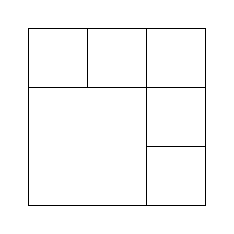
\begin{tikzpicture}[scale=.75]
    \draw (0,0) rectangle (3,3) (0,0) rectangle (2,2) (1,2) -- (1,3) (2,2) -- (2,3) (2,2) -- (3,2) (2,1)-- (3,1);
  \end{tikzpicture}
\end{center}
Prove, using strong induction, that it is possible to cut a square into $n$ smaller squares for any $n \ge 6$.  Hint: you will need three base cases.

\begin{solution}
  \begin{proof}
    For each $n$, let $P(n)$ be the statement ``You can divide a square into $n$ smaller squares.''  We will prove $P(n)$ is true for all $n \ge 6$ using strong induction.

    First note that you can divide a square into $6$, $7$, or $8$ squares as follows:

    \begin{center}
      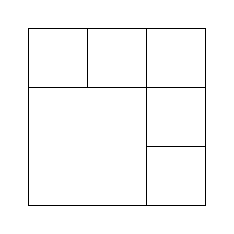
\begin{tikzpicture}[scale=.75]
        \draw (0,0) rectangle (3,3) (0,0) rectangle (2,2) (1,2) -- (1,3) (2,2) -- (2,3) (2,2) -- (3,2) (2,1)-- (3,1);
      \end{tikzpicture}
      \qquad
      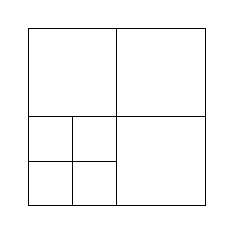
\begin{tikzpicture}[scale=.75]
      \draw (0,0) rectangle (3,3) (0,1.5) -- (3,1.5) (1.5,0) -- (1.5,3) (0.75,0) -- (0.75, 1.5) (0, 0.75) -- (1.5, 0.75);
    \end{tikzpicture}
    \qquad
      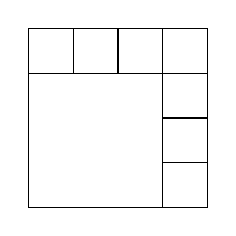
\begin{tikzpicture}[scale=.57]
        \draw (0,0) rectangle (4,4) (3,0) rectangle (4,1) rectangle (3,2) rectangle (4,3) rectangle (3,4) rectangle (2,3) rectangle (1,4) rectangle (0,3);
      \end{tikzpicture}
    \end{center}


    Now consider an arbitrary $n > 8$ and suppose you can divide a square into $k$ squares, for any $6 \le k < n$.  Then in particular, you can divide a square into $n-3$ squares.  Take any one of the small sqaures and divide it into 4.  This replaces one of the squares with 4 new ones, increasing the total by 3, giving you $n$ squares.

    Therefore, by the principle of strong mathematical induction, you can divide a square into $n$ squares for any $n \ge 6$.
  \end{proof}
\end{solution}

\end{questions}



\begin{questions}
  \question[4] Tommy Flanagan was telling you what he ate yesterday afternoon.  He tells you, ``I had either popcorn or raisins.  Also, if I had cucumber sandwiches, then I had soda.  But I didn't drink soda or tea.''  Of course you know that Tommy is the worlds worst liar, and everything he says is false.  What did Tommy eat?

  Justify your answer by writing all Tommy's statements using sentence variables ($P, Q, R, S, T$), taking their negations, and using these to deduce what Tommy actually ate.

  \begin{solution}
  Let $P$ be the statement, ``I had popcorn,'' $Q$ be the statement, ``I had cucumber sandwiches,'' $R$ be the statement, ``I had raisins,'' $S$ be, ``I had soda,'' and $T$ be, ``I had tea.''  Then the statements made by Tommy are:
  \[P \vee R \qquad Q \imp S \qquad \neg(S \vee T)\]
  We need the negation of all of these.  Thus what is true is:
  \[\neg P \wedge \neg R \qquad Q \wedge \neg S \qquad S \vee T\]
  From the first two statements we can conclude that Tommy did not eat popcorn, did not eat raisins, did eat cucumber sandwiches and did not drink soda.  From the last statement $S \vee T$ and the fact that we know $\neg S$ we can conclude $T$, so Tommy did drink tea.
  \end{solution}





  \question[8] Use De Morgan's Laws, and any other logical equivalence facts you know to simplify the following statements.  Show all your steps.  Your final statements should have negations only appear directly next to the sentence variables ($P$, $Q$, etc.), and no double negations.  It would be a good idea to use only conjunctions, disjunctions, and negations.
  \begin{parts}
    \part $\neg((\neg P \wedge Q) \vee \neg(R \vee \neg Q))$.
    \begin{solution}
      $\neg((\neg P \wedge Q) \vee \neg(R \vee \neg Q))$\\
      $\neg(\neg P \wedge Q) \wedge \neg\neg(R \vee \neg Q)$ by De Morgan's law.\\
      $\neg(\neg P \wedge Q) \wedge (R \vee \neg Q)$ by double negation.\\
      $(\neg\neg P \vee \neg Q) \wedge (R \vee \neg Q)$ by De Morgan's law.\\
      $(P \vee \neg Q) \wedge (R \vee \neg Q)$ by double negation.
    \end{solution}

    \part $\neg((\neg P \imp \neg Q) \wedge (\neg Q \imp R))$ (careful with the implications).
    \begin{solution}
      We will need to convert the implications to disjunctions so we can apply De Morgan's law:

      $\neg((\neg P \imp \neg Q) \wedge (\neg Q \imp R))$\\
      $\neg((\neg \neg P \vee \neg Q) \wedge (\neg\neg Q \vee R))$ by implication/disjunction equivalence.\\
      $\neg((P \vee \neg Q) \wedge (Q \vee R))$ by double negation.\\
      $\neg(P \vee \neg Q) \vee \neg (Q \vee R)$ by De Morgan's law.\\
      $(\neg P \wedge \neg \neg Q) \vee (\neg Q \wedge \neg R)$ by De Morgan's law.\\
      $(\neg P \wedge Q) \vee (\neg Q \wedge \neg R)$ by double negation.
    \end{solution}

    \part For both parts above, verify your answers are correct using truth tables.  That is, use a truth table to check that the given statement and your proposed simplification are actually logically equivalent.

    \begin{solution}
      For each truth table, the columns for the original statement and the simplified statement must be identical.  They are.  For purposes of checking your work, here are the final columns for the two parts above:

      \begin{tabular}{c|c|c||c|c}
        $P$ & $Q$ & $R$ & (a) & (b) \\ \hline
        T   &  T  &  T  &         T         &      F     \\
        T   &  T  &  F  &         F         &      F     \\
        T   &  F  &  T  &         T         &      F     \\
        T   &  F  &  F  &         T         &      T     \\
        F   &  T  &  T  &         F         &      T     \\
        F   &  T  &  F  &         F         &      T     \\
        F   &  F  &  T  &         T         &      F     \\
        F   &  F  &  F  &         T         &      T     \\
      \end{tabular}
    \end{solution}

   \part $\neg \forall x \exists y ((E(x) \vee \neg O(y)) \imp \exists z (E(z) \wedge E(y)))$. Here, also put all the quantifiers ``out front.''
   \begin{solution}
   FIX
   \end{solution}
  \end{parts}


\question[8] Determine whether the following are valid deduction rules.  Your answer should involve a truth table as well as an explanation of what your truth table tells you.
\begin{multicols}{2}
\begin{parts}
  \part ~\\ \begin{tabular}{cc}
  & $P \imp (Q \vee R)$ \\
  & $\neg (P \imp Q)$ \\ \hline
  $\therefore$ & $R$
  \end{tabular}
  \columnbreak
  \part ~\\ \begin{tabular}{cc}
  & $(P \wedge Q) \imp R$ \\
  & $\neg P \vee \neg Q$ \\ \hline
  $\therefore$ & $\neg R$
  \end{tabular}
\end{parts}
\end{multicols}

\begin{solution}
  \begin{parts}
    \part Here is a truth table that includes all the statements:

        \begin{tabular}{c|c|c||c|c}
          $P$ & $Q$ & $R$ & $P\imp (Q\vee R)$ & $\neg(P \imp Q)$  \\ \hline
          T   &  T  &  T  &         T         &      F     \\
          T   &  T  &  F  &         T         &      F     \\
          T   &  F  &  T  &         T         &      T     \\
          T   &  F  &  F  &         F         &      T     \\
          F   &  T  &  T  &         T         &      F     \\
          F   &  T  &  F  &         T         &      F     \\
          F   &  F  &  T  &         T         &      F     \\
          F   &  F  &  F  &         T         &      F     \\
        \end{tabular}

        Notice that there is only one row in which both premises are true (row 3).  In this row, $R$ is also true.  So whenever the premises are true, so is the conclusion.  Thus this is a valid deduction rule.

        \part Here is the truth table for this proposed rule:

      \begin{tabular}{c|c|c||c|c|c}
        $P$ & $Q$ & $R$ & $(P \wedge Q) \imp R$ & $\neg P \vee \neg Q$ & $\neg R$ \\ \hline
        T   &  T  &  T  &           T            &           F         &   F \\
        T   &  T  &  F  &           F            &           F         &   T \\
        T   &  F  &  T  &           T            &           T         &   F \\
        T   &  F  &  F  &           T            &           T         &   T \\
        F   &  T  &  T  &           T            &           T         &   F \\
        F   &  T  &  F  &           T            &           T         &   T \\
        F   &  F  &  T  &           T            &           T         &   F \\
        F   &  F  &  F  &           T            &           T         &   T \\
      \end{tabular}

      Now look at rows 3. 5 and 7.  In each of these (one would be enough) both premises are true.  However, here the conclusion is false.  Thus this is NOT a valid deduction rule.  In fact, we can see exactly where it goes wrong: If $P$ or $Q$ is false and $R$ is true, we get a counterexample, since $Q$ being false makes both premises true no matter what $R$ is.
  \end{parts}
\end{solution}


  \question[8] Can you chain implications together?  That is, if $P \imp Q$ and $Q \imp R$, does that means the $P \imp R$?  Can you chain more implications together?  Let's find out:
  \begin{parts}
    \part Prove that the following is a valid argument form:
    \begin{tabular}{rc}
      & $P \imp Q$ \\
      & $Q \imp R$ \\ \hline
      $\therefore$ & $P \imp R$
    \end{tabular}

    \begin{solution}
      Consider the truth table:

      \begin{tabular}{c|c|c||c|c|c}
        $P$ & $Q$ & $R$ & $P\imp Q$ & $Q \imp R$ & $P \imp R$ \\ \hline
        T   &  T  &  T  &     T     &      T     &      T \\
        T   &  T  &  F  &     T     &      F     &      F \\
        T   &  F  &  T  &     F     &      T     &      T \\
        T   &  F  &  F  &     F     &      T     &      F \\
        F   &  T  &  T  &     T     &      T     &      T \\
        F   &  T  &  F  &     T     &      F     &      T \\
        F   &  F  &  T  &     T     &      T     &      T \\
        F   &  F  &  F  &     T     &      T     &      T \\
      \end{tabular}
      Notice that both $P \imp Q$ and $Q \imp R$ are true in rows 1, 5, 7 and 8.  In each of these rows, $P \imp R$ is also true.  So whenever the premises are true, so in the conclusion.  Thus the argument form is valid.
    \end{solution}


  \part Prove that the following is a valid argument form for any $n \ge 2$:
  \begin{tabular}{rc}
    & $P_1 \imp P_2$\\
    & $P_2 \imp P_3$ \\
    & $\vdots$ \\
    & $P_{n-1} \imp P_n$ \\ \hline
    $\therefore$ & $P_1 \imp P_n$.
  \end{tabular}

  I suggest you don't go through the trouble of writing out a $2^n$ row truth table.  Instead, you should use part (a) and mathematical induction.
  \begin{solution}
  Part (a) is the base case.  Now assume that the deduction rule holds going up to $P_k$.  That is,

  \begin{tabular}{rc}
    & $P_1 \imp P_2$\\
    & $P_2 \imp P_3$ \\
    & $\vdots$ \\
    & $P_{k-1} \imp P_k$ \\ \hline
    $\therefore$ & $P_1 \imp P_k$.
  \end{tabular}

  Now suppose we have

  \begin{tabular}{rc}
    & $P_1 \imp P_2$\\
    & $P_2 \imp P_3$ \\
    & $\vdots$ \\
    & $P_{k-1} \imp P_k$ \\
    & $P_k \imp P_{k+1}$
  \end{tabular}

  From the first $k-1$ lines, we can conclude $P_1 \imp P_k$.  The combining this with the last line, we can conclude (using part (a) again):

  \begin{tabular}{rc}
    & $P_1 \imp P_k$\\
    & $P_{k} \imp P_{k+1}$ \\ \hline
    $\therefore$ & $P_1 \imp P_{k+1}$.
  \end{tabular}

  So

  \begin{tabular}{rc}
    & $P_1 \imp P_2$\\
    & $P_2 \imp P_3$ \\
    & $\vdots$ \\
    & $P_{k-1} \imp P_k$ \\
    & $P_k \imp P_{k+1}$\\ \hline
    $\therefore$ & $P_1 \imp P_{k+1}$.
  \end{tabular}
  \end{solution}

  \end{parts}



  \question[4] Your ``friend'' has shown you a ``proof'' he wrote to show that $1 = 3$.  Here is the proof:

  \begin{proof}
  I claim that $1 = 3$.  Of course we can do anything to one side of an equation as long as we also do it to the other side.  So subtract 2 from both sides.  This gives $-1 = 1$.  Now square both sides, to get $1 = 1$.  And we all agree this is true.
  \end{proof}

  What is going on here?  Is your friends argument valid?  Is the argument a proof of the claim $1=3$?  Carefully explain using what we know about logic.  Hint: What implication follows from the given proof?

  \begin{solution}
  In the proof we assume that $1=3$ and conclude that $1=1$.  So we have proved the implication
  \[1=3 \imp 1=1\]
  Note that we actually have a valid proof of this, and that the implication is true (for one thing, the ``if'' part is false, so the implication is automatically true).  However, what we really want is to converse of this, that $1=1 \imp 1=3$.  But as we know, the converse is not implied by the original implication (it better not be, otherwise we could conclude that 1 actually was 3).

  Another way to say this: we can never conclude anything about the ``if'' part of an implication, since the ``if'' part can be true or false even if the implication is true.
  \end{solution}


  \question[6] Consider the statement, ``If a number is triangular or square, then it is not prime''
  \begin{parts}
    \part Make a truth table for the statement $(T \vee S) \imp \neg P$.
    \part If you believed the statement was \emph{false}, what properties would a counterexample need to possess?  Explain by referencing your truth table.
    \part If the statement were true, what could you conclude about the number 5657, which is definitely prime?  Again, explain using the truth table.
  \end{parts}

\begin{solution}
  \begin{parts}
    \part    \begin{tabular}{c|c|c||c}
            $T$ & $S$ & $P$ & $(T\vee S) \imp \neg P$  \\ \hline
            T   &  T  &  T  &             F     \\
            T   &  T  &  F  &             T     \\
            T   &  F  &  T  &             F     \\
            T   &  F  &  F  &             T     \\
            F   &  T  &  T  &             F     \\
            F   &  T  &  F  &             T     \\
            F   &  F  &  T  &             T     \\
            F   &  F  &  F  &             T     \\
          \end{tabular}

    \part There are three cases in which the statement is false: rows 1, 3 and 5.  So one way to prove this was false would be to find a number that was triangular, square and prime (row 1).  Or you could find a number that was triangular, not square, and prime (row 3) or one that is not triangular, is square and is not prime (row 5).  In fact, since no square number is prime, we would need to do the second one (3 is both triangular and prime, but in fact this is the only one).
    \part Here we have a prime number, so we need to look at rows in which $P$ is true.  We also need to statement to be true.  There is only one row with both these properties: row 7.  And here we see that $T$ and $S$ are both false.  So we would know that 5657 is neither triangular nor square.
  \end{parts}
\end{solution}



  \question[5] \textbf{Bonus:} You come across four trolls playing bridge.  As you know, all trolls belong to one of two clans: knights, who always tell the truth, or knaves, who always lie.  They declare:
  \begin{itemize}
  \item[] Troll 1: All trolls here see at least one knave.

  \item[] Troll 2: I see at least one troll that sees only knaves.

  \item[] Troll 3: Some trolls are scared of goats.

  \item[] Troll 4: All trolls are scared of goats.
  \end{itemize}

  Are there any trolls that are not scared of goats?  Justify your answer.

  \begin{solution}
  Consider first the statement of Troll 2.  If this were true, then Troll 2 would be a knight.  But the troll he sees that sees only knaves would see him, a knight.  Thus Troll 2 is a knave.  This also means that his statement is false.  In other words, every troll he sees, sees at least one knight.

  Now consider Troll 1's statement.  If this were false, that would mean that there was a troll that saw only knights.  That would have to be Troll 2 (since he is a knave), but Troll 2 sees Troll 1, also a knave.  Thus Troll 1's statement is true, and he is knight.  Also, since his statement is true, everyone sees at least one knave.

  Note that since every troll sees at least one knight (including the knights) and every troll sees at least one knave (including the knaves) there must be exactly two knights and two knaves.

  So among trolls 3 and 4, one is a knight and one is a knave.  The only way this can happen is if Troll 3 is a knight and Troll 4 is a knave (if all trolls are scared of goats, then some are as well).

  In particular, it is false that all trolls are scared of goats, so some strolls are not scared of goats.


  \end{solution}

\end{questions}


\begin{questions}

  \question[9] Suppose that you would like to prove the following implication:
  \begin{center}
  ``For all numbers $n$, if $n$ is prime then $n$ is solitary.''
  \end{center}
  Write out the beginning and end of the argument if you were to prove the statement,
  \begin{parts}
  \part Directly
  \begin{solution}
  To prove the above statement using a direct proof we would need to start by  assuming that $n$ is a prime number then using logic, logic, logic,... we could conclude that $n$ is solitary.
  \end{solution}
  \part By contrapositive
  \begin{solution}
  To prove by contrapositive: Assume $n$ is not solitary (logic, logic, logic...) and conclude that $n$ is not prime.
  \end{solution}
  \part By contradiction
  \begin{solution}
  To prove using a proof by contradiction: Assume that $n$ is prime and that $n$ is not solitary (logic, logic, logic...) then either $n$ is not prime or $n$ is solitary (you need to contradict one of your assumptions). Therefore, if $n$ is prime then $n$ is solitary.
  \end{solution}
  \end{parts}
  You do not need to provide details for the proofs (since you do not know what solitary means). However, make sure that you provide the first few and last few lines of the proofs so that we can see that logical structure you would follow.



  \question[9] A standard deck of 52 cards consists of 4 suites (hearts, diamonds, spades and clubs) each containing 13 different values (Ace, 2, 3, \ldots, 10, J, Q, K).  If you draw some number of cards at random you might or might not have a pair (two cards with the same value) or three cards all of the same suit.  However, if you draw enough cards, you will be guaranteed to have these.  For each of the following, find the smallest number of cards you would need to draw to be guaranteed having the specified cards.  \underline{Prove your answers} (and specify what sort of proof you are using).
  \begin{parts}
  \part Three of a kind (for example, three 7's).
  \begin{solution}
  The smallest number of cards you must draw is 27.  If you drew 26, you could have two of each value, and as such not have three of a kind.  To prove that 27 cards guarantees a three of a kind, we give a proof by contrapositive.

  Suppose you do not have a three of a kind.  Then you have at most two of each value, so at most 26 cards.  Thus you do not have 27 cards.

  \end{solution}
  \part A flush of five cards (for example, five hearts).
  \begin{solution}
    The smallest number of cards needed is 17.  If you had 16 cards, you could have 4 of each suit.  In fact, if you did not have a flush of five cards, you could have at most 4 of each suit, for only 16 cards.  Thus you don't have 17 cards.

  \end{solution}
  \part Three cards that are either all the same suit or all different suits.
  \begin{solution}
  You must pick 5 cards.  If you picked just 4, you could have two hearts and two spades.  However, given any 5 cards, we can be sure that at least two of them will be the same suit, say hearts.  Of the remaining three cards, if any of them are also a heart, we will have three hearts.  If not,  there are two cases to consider.  Either all three cards will be of the same suit (in which case we would have three cards of the same suit) or else two suits will be present among the three cards.  But those two other suits are not hearts, so those two cards plus one of the hearts will form a set of three cards of all different suits.

  An alternative proof: suppose you did not have three cards all the same or all different.  Then you can have at most two cards of any given suit, and at most two suits.  This is at most 4 cards.
  \end{solution}
  \end{parts}



  \question[6] Suppose you are at a party with 19 of your closest friends (so including you, there are 20 people there).  Explain why there must be least two people at the party who are friends with the same number of people at the party.  Assume friendship is always reciprocated.

  \begin{solution}
    Suppose this was not the case.  That is, suppose everyone at the party had a {\em different} number of friends.  What could these numbers be.  Any give person at the party could have between 0 and 19 friends at the party.  This is 20 numbers, but we can't have all of these numbers occur at the same party.  If someone is friends with 19 people, then she is friends with everyone, including the person who is supposedly friends with 0 people.  Thus there are only 19 values for the number of friends people can have, so two people must have the same number of friends.

    What this says is that in any graph with 20 vertices, there must be at least two vertices which have the same degree.
  \end{solution}


  \question[6] Consider the following two graphs:\\
  $G_1$: $V_1=\{a,b,c,d,e,f,g\}$, $E_1=\{\{a,b\},\{a,d\},\{b,c\},\{b,d\},\{b,e\},\{b,f\},\{c,g\},\{d,e\},\{e,f\},\{f,g\}\}$.\\
  $G_2$: $V_2=\{v_1,v_2,v_3,v_4,v_5,v_6,v_7\}$,

  \hspace{1.75em} $E_2=\{\{v_1,v_4\},\{v_1,v_5\},\{v_1,v_7\},\{v_2,v_3\},\{v_2,v_6\},\{v_3,v_5\},\{v_3,v_7\},\{v_4,v_5\},\{v_5,v_6\},\{v_5,v_7\}\}$.
  \begin{parts}
  \part Let $f:G_1 \rightarrow G_2$ be a function that takes the vertices of Graph 1 to vertices of Graph 2.  The function is given by the following table:

  \begin{center}
  \begin{tabular}{c*{7}{|c}}
  $x$ & $a$ & $b$ & $c$ & $d$ & $e$ & $f$ & $g$ \\ \hline
  $f(x)$ & $v_4$ & $v_5$ & $v_1$ & $v_6$ & $v_2$ & $v_3$ & $v_7$
  \end{tabular}
  \end{center}
  %
  %\[f(a)=v_4\]
  %\[f(b)=v_5\]
  %\[f(c)=v_1\]
  %\[f(d)=v_6\]
  %\[f(e)=v_2\]
  %\[f(f)=v_3\]
  %\[f(g)=v_7\]
  Is $f$ an isomorphism between Graph 1 and Graph 2? Explain.
  \begin{solution}
  Recall that in order for $f$ to be an isomorphism between $G1$ and $G2$, it must preserve relationships between vertices. To put this into context, this means that since $a$ and $b$ are joined via an edge in $G1$ that their corresponding vertices in $G2$ must also be joined by an edge. This must be true for all of the vertices and edges. When examining the function, we can see that the vertex $g$ goes to $v_7$, that is $f(g)=v_7$. BUT, $g$ has exactly 2 edges (so $g$ is degree 2) and $v_7$ is degree 3. This means that $f$ cannot possibly be an isomorphism. Similarly, we can see that $f$ does not take $c$ to the correct vertex either $c$ is degree 2 and $v_1$ has degree 3.
  \end{solution}
  \part Define a function $g$ (different from $f$) that \emph{is} an isomorphism between Graph 1 and Graph 2.
  \begin{solution}
  \begin{center}
  \begin{tabular}{c*{7}{|c}}
  $x$ & $a$ & $b$ & $c$ & $d$ & $e$ & $f$ & $g$ \\ \hline
  $g(x)$ & $v_4$ & $v_5$ & $v_6$ & $v_1$ & $v_7$ & $v_3$ & $v_2$
  \end{tabular}
  \end{center}
  \end{solution}
  \part Is the graph pictured below isomorphic to Graph 1 and Graph 2? Explain.
  \begin{center}
  \begin{tikzpicture}
  \draw (-1, 0) coordinate (v1) -- (0,0) coordinate (v2) -- (1,0) coordinate (v3) -- (1,1) coordinate (v4) -- (0,1) coordinate (v5) -- (-1,1) coordinate (v6) -- (v1) --(0,.5) coordinate (v7) -- (v2) (v7) -- (v3) (v7) -- (v5);
  \foreach \i in {1,...,7}{
  	\fill (v\i) \v;
  }
  \end{tikzpicture}
  \begin{solution}
  No, it could not possibly be isomorphic. If you count up the degrees of each vertex in this picture, you can see that the highest degree is 4 (the center vertex). In order to be isomorphic to either $G1$ or $G2$ we would definitely need a vertex of degree 5, which we don't have.
  \end{solution}

  \end{center}

  \end{parts}


  \question[4] Bonus: Suppose a $n\times n$ chessboard is missing two opposite corners.  Prove that no matter what $n$ is, you will not be able to cover the remaining squares exactly with dominoes.

  \begin{center}
  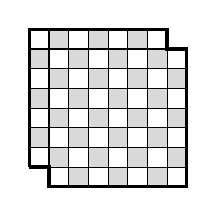
\begin{tikzpicture}[scale=.25]
  \foreach \x in {0,2,...,6}{
  	\foreach \y in {0,2,...,6}{
  \draw[fill=white!85!black] (\x,\y) rectangle (\x+1, \y+1) rectangle (\x+2,\y+2);
  }}
  \draw (0,0) grid (8,8);
  \draw[white, fill=white] (7,7) rectangle (8,8) (0,0) rectangle (1,1);
  \draw[very thick] (0,1) -- (1,1) -- (1,0) -- (8,0) --(8,7) -- (7,7) -- (7,8) -- (0,8) -- (0,1);
  \end{tikzpicture}
  \end{center}

  \begin{solution}
  If $n$ is odd, then $n^2$ is odd, as is $n^2 - 2$.  Thus it would be impossible to cover the board with dominoes.  If $n$ is even, then this is not an issue any more.  However, notice that the opposite squares are the same color, so removing them would result in more squares of one color than the other.  Every domino needs to cover two adjacent squares, so one square of each color.  Thus any attempt two cover the board with dominoes will result in two uncovered squares (of the color you have more of).
  \end{solution}
\end{questions}


\begin{questions}
  \question[9] A convex polyhedron is a 3 dimensional geometric figure made up of faces, each of which is a polygon.  Thus a polyhedron has a number of faces, edges and vertices, just like a planar graph.  In fact, you can represent every convex polyhedron as a planar graph.  (``Convex'' means that the interior angle between any two faces is less then $180^\circ$.)
  \begin{parts}
  \part An {\em octahedron} is a regular polyhedron made up of 8 equilateral triangles (it sort of looks like two square-based pyramids with their bases glued together).  Draw a planar graph representation of an octahedron.  How many vertices, edges and faces does an octahedron (and your graph) have?  It might be helpful to decide on these numbers before drawing the graph.
  \begin{solution}
  Since there are 8 triangles, there must be 8 faces.  We can count the number of edges by taking $8 \cdot 3 = 24$, but this is double counting since each edge corresponds to two faces.  Thus there are 12 edges.  We can use Euler's formula to find that there are 6 vertices (and this shows that each vertex is the joining of 4 triangles).

  The planar representation of the graph is:



  \begin{center}
  \begin{tikzpicture}
  \coordinate (a) at (30:2);
  \coordinate (b) at (150:2);
  \coordinate (c) at (270:2);
  \coordinate (d) at (90:.5);
  \coordinate (e) at (210:.5);
  \coordinate (f) at (-30:.5);
  \draw[thick] (a) \v -- (b) \v -- (c) \v -- (a) -- (d)\v --(e)\v -- (f)\v --(d) -- (b) -- (e) -- (c) -- (f) -- (a);

  \end{tikzpicture}
  \end{center}


  \end{solution}
  \part The traditional design of a soccer ball is in fact a (spherical projection of a) truncated icosahedron.  This consists of 12 regular pentagons and 20 regular hexagons.  No two pentagons are adjacent (so the edges of each pentagon are shared only by hexagons).  How many vertices, edges, and faces does a truncated icosahedron have?  Explain how you arrived at your answers.  Bonus: draw the planar graph representation of the truncated icosahedron.
  \begin{solution}
  Well, right off we know that the truncated icosahedron has $12+20=32$ faces by counting the number of pentagons and hexagons. Now, because we know that every connected planar graph with $v$ vertices, $e$ edges and $f$ faces satisfied $v - e + f = 2$, we only really need to find out the number of edges or the number of vertices since $v-e=-30$. So, let's maybe try to figure out the number of edges we have. If we think about the number of total edges when the pentagons and hexagons are not attached, we know that we have $5\times 12+6\times 20=180$. But each of these edges is shared with another edge, which means that we have cut the number of edges in half. So, we have $90$ edges, which then gives us $60$ vertices.
  \end{solution}
  \part Your ``friend'' claims that he has constructed a convex polyhedron out of 2 triangles, 2 squares, 6 pentagons and 5 octagons.  Prove that your friend is lying.  Hint: each vertex of a convex polyhedron must border at least three faces.
  \begin{solution}
  So, let's assume for a contradiction that your friend really has constructed a convex polyhedron. Then, we would know that the polyhedron has $15$ faces, $(2\times 3+2\times 4+6\times 5+5\times 8)/2 = 42$ edges, and $v=2+42-15=29$ vertices. Now, using the hint, we also know that the degree of each vertex is at least 3, and the number of edges is half the sum of the degrees.  Thus we have $3v\leq 2e$ but $3\cdot 29$ is not in fact less than $2 \cdot 42$. So we have a contradiction, and your friend is lying.
  \end{solution}
  \end{parts}

  \question[6] Prove that the {\em Petersen graph} (below) is not planar.  Hint: what is the length of the shortest cycle?

  \begin{center}
    \begin{tikzpicture}[scale=.5]
      \draw[thick] (18:2) -- (90:2) -- (162:2)  -- (234:2) -- (306:2) -- cycle;
      \draw[thick] (18:1) --  (162:1)  -- (306:1) -- (90:1) -- (234:1) --cycle;
      \foreach \x in {18, 90, 162, 234, 306}
      \draw[thick] (\x:1) \v -- (\x:2) \v;
    \end{tikzpicture}
  \end{center}

  \begin{solution}
    \begin{proof}
      Suppose, for contradiction, that the Petersen graph were planar.  Then it would satisfy Euler's formula: $v - e + f = 2$.  Since the graph has 10 vertices and 15 edges, this says that there must be $7$ faces.

      Now let $b$ be the total number of boundaries around all faces when the graph is drawn in a planar way.  Since each edge is used in two boundaries we have $b = 2e$.  On the other hand, each face is surrounded by {\em at least} 5 boundaries, since the shortest cycle (circuit) in the graph contains 5 edges.  Thus $f \le \frac{b}{5}$.  Putting these two facts together we get
      \[f \le \frac{2e}{5}\]
      This is a contradiction, since $7 \not\le \frac{2\cdot 30}{5}$.  Alternatively, the above relationship says that $f \le 6$, but we said $f = 7$ above.

      Therefore the Petersen graph is not planar.
    \end{proof}

  \end{solution}


  \question[9] A {\em tree} is a connected graph with no cycles.
  \begin{parts}
  \part Draw a bunch of trees.  Conjecture a relationship between a the number of vertices and edges in any tree. (For instance, can you have a tree with 5 vertices and 7 edges?)
  \begin{solution}
  After drawing a few trees, you should notice that there is always exactly one more vertices than edges. That is $v=e+1$
  \end{solution}
  \part Explain why every tree with at least 3 vertices has at least one vertex with degree 1 (such a vertex is called a \emph{leaf}.  Hint: try a proof by contradiction.
  \begin{solution}
  Assume for a contradiction that every tree with at least 3 vertices does not have a leaf. Namely, that there are no vertices of degree 1. Then, every vertex must have a degree of 2 or more, but this would imply that we have a cycle! Why? Think about taking a path from one vertex to another. Choose the first vertex and a route to leave it (remember it should have at least two ways to leave). Once I leave that vertex I reach another vertex which also has at least one more way to leave. Keep doing this. Eventually you will get back to one of the vertices that you have already visited and therefore you will have completed a cycle.
  \end{solution}
  \part Prove your conjecture from part (a) by \underline{induction} on the number of vertices. Hint: For the inductive step, you will assume that your conjecture is true for all trees with $k$ vertices, and show it is also true for an arbitrary tree with $k+1$ vertices.  So start with an arbitrary tree with $k+1$ vertices.  Consider what happens when you cut off a leaf and then let it regrow.
  \begin{solution}
  Recall that we need two parts for an induction proof: a base case and an inductive case.
  \begin{proof}
  Let $P(n)$ be the statement ``a tree $T_n$ with $n$ vertices has $n-1$ edges.''
  Base Case: Draw a tree with three vertices. Clearly you have only 2 edges (otherwise you would have a cycle).\\
  Inductive Case: Assume $P(k)$ is true for some arbitrary $3<k<n$.\\
  NTS: $P(k+1)$ is true. That is $T_{k+1}$ has $k$ edges.\\
  Let $T_{k+1}$ be a tree graph with $k+1$ vertices. By part (b) we know that every tree with at least 3 vertices has a leaf, so cut that one leaf off of $T_{k+1}$. Then our tree graph has only $k$ vertices, and by our inductive case has $k-1$ edges. Well, if we let that leaf regrow we will add both one edge and one vertex, which means that we will have a tree graph with $k+1$ vertices and $k-1+1=k$ edges. TBTPOMI we have shown that $P(n)$ is true.
  \end{proof}
  \end{solution}
  \end{parts}



 \question[6] The two problems below can be solved using graph coloring.  For each problem, represent the situation with a graph, say whether you should be coloring vertices or edges and why, and use the coloring to solve the problem.
 \begin{parts}
   \part Your Quidditch league has 5 teams.  You will play a tournament next week in which every team will play every other team once.  Each team can play at most one match each day, but there is plenty of time in the day for multiple matches.  What is the fewest number of days over which the tournament can take place?

   \begin{solution}
     The graph to represent this question is $K_5$, since each vertex (team) is adjacent to (plays) each other vertex (team).  The edges are thus the games that are played.  We cannot have a team play more than one game per day, so we color the edges observing the rule that two edges incident to the same vertex must be colored differently.  Edges that are colored the same \emph{can} be played on the same day, so we are looking for the smallest number of colors needed to color the edges in this way.  You obviously need at least 4 colors, but this does not work.  In fact, there is a coloring using 5 colors, so you need 5 days for the tournament.
   \end{solution}
   \part Ten members of Math Club are driving to a math conference in a neighboring state.  However, some of these students have dated in the past, and things are still a little awkward.  Each student lists which other students they refuse to share a car with; these conflicts are recored in the table below.  What is the fewest number of cars the club needs to make the trip?  Do not worry about running out of seats, just avoid the conflicts.

   \begin{tabular}{l|*{10}{c}}
     Student: & A & B & C & D & E & F & G & H & I & J \\ \hline
     Conflicts: &BEJ&ADG&HJ&BF&AI&DJ&B&CI&EHJ&ACFI
   \end{tabular}
   \begin{solution}
     Here we color the vertices.  The chromatic number of this graph is 3, so three cars are needed.
   \end{solution}
 \end{parts}



\end{questions}


\begin{questions}


%Replace with 3-part pie counting problem?  This is too easy.
\question[6] Fifth grade students at a local elementary school took a poll about how they got to school. Many students took multiple modes of transportation with 31 students saying they got rides from their parents, 32 taking their bike to school and 21 walking. 8 students who said they bike also walk, and 3 students who usually walk get rides from their parents on some mornings. The one student that said he uses his bike and gets ride also said he uses all three modes of transportation.
\begin{parts}
\part Draw a Venn diagram of this situation.
\begin{solution}
	\begin{center}
	\includegraphics[height=2 in, width=2 in]{venndiagramh12}
	\end{center}
\end{solution}
\part How many students took the survey?
\begin{solution}
	Adding up all the values in the Venn diagram we get that there were 73 students who took the survey.
\end{solution}
\part How does this problem relate to PIE?
\begin{solution}
	Remember that PIE is the principle of inclusion/exclusion and this problem relates because we want to calculate the total number of students who took the survey but we can't just add up all the numbers in the problem because we would be counting certain students multiple times. So, this means that when we are looking at this problem we need to follow the principle for 3 different sets which gives us: \[|A\cup B \cup C|=|A|+|B|+|C|-|A\cap B|-|A\cap C| - |B \cap C|+|A\cap B\cap C|\]
So, we could have just looked at the problem and related each set of students to each $A, B, C$ where $A\cap B$ is the number of students who did both $A$ and $B$ to get to school.
\end{solution}
\end{parts}


\question[4] My circular kitchen table has 4 chairs (and we will assume the position of these chairs is important; one is facing away from the TV, for example).  Before our second kid, when we ate dinner, my wife and I sat across from each other and our daughter sat in the chair between us on my right (the chair to my left was empty).
\begin{parts}
  \part Occasionally, my daughter wanted us to sit in different chairs than usual.  For example, she would want to sit in my seat, want me to sit in my wife's seat, and my wife to sit in the chair that is usually empty.  How many different seating arrangements are possible?  Explain your answer carefully.
  \begin{solution}
    There are 4 chairs for my daughter to sit in, then 3 for my wife, and 2 for me.  So there are $4\cdot 3 \cdot 2 = 24$ seating arrangements.  Note this is simply $P(4,3)$.
  \end{solution}
  \part When she was feeling especially toddler-like, she would insist that none of us sit in our regular chairs.  How many of the seating arrangements you found in the previous part have this property?  Explain.
  \begin{solution}
    Let's say the normal arrangement of seats is ESMO (empty, Shannon, Maddie, Oscar).  It would not be too difficult to list all of the acceptable seating arrangements here.  In fact, we could list all 24, and cross out any that have one or more people in their usual seats.  Note that it is okay for E to be in the first spot, but S must be in a spot other than the second, M must be in spot other than the third, and O must be in a spot other than the 4th.  This is the list we would be left with:
    \[ EMOS, EOSM, SEOM, SOEM, SMOE, MEOS, MOES, MOSE, OESM, OMES, OMSE\]
    If you wanted to count this using our counting techniques, you could use PIE.  Count the number of \emph{unacceptable} arrangements and subtract that from 24:
    \[24-\left[3\cdot 2 + 3 \cdot 2 + 3 \cdot 2 - 2 - 2 - 2 + 1\right] = 11.\]
    Here each $3\cdot 2$ counts the number of ways that the other two people can sit if one person sits in their usual seat, the 2's count the number of choices for the last person when two people sit in their usual seat, and the 1 is the number of arrangements when all three people sit in their usual seat.
  \end{solution}
\end{parts}


\question[6] Consider bit strings.  Note that all the answers below should be easy to count directly by listing them, but you are asked to show how you can use the Principle of Inclusion/Exclusion to complete the problem.
\begin{parts}
  \part Use PIE to count the number of 5-bit strings of weight 4 that either start with 111 or end with 111 (or both).  Explain each part of your expression and why they are combined the way they are.
  \begin{solution}
    There are ${2 \choose 1}$ strings that start with 111 (two spots left, one of which must be a 1), ${2 \choose 1}$ strings that end with 111, and 0 strings that both start and end with 111.  Thus all together there are $2 + 2 - 0 = 4$ strings.
  \end{solution}
  \part Use PIE to count the number of 5-bit strings of weight 4 that contain 111 somewhere in them (which will be at the start, in the middle, at the end or more than one of these).
  \begin{solution}
    Start with 111: 2. Have 111 in the middle: 2.  End with 111: 2.  Start with 111 and have 111 in the middle: 1.  Have 111 in the middle and end with 111: 1.  Start and end with 111: 0.  All three: 0.  Thus
    \[2 + 2 + 2 - 1 -1 - 0 + 0 = 4\]
  \end{solution}
  \part Generalize PIE to 4 sets to count the number of 6-bit strings of weight 5 that contain 111 somewhere in them.
  \begin{solution}
    Consider the 4 positions the 111 string can occur: (a) first three bits, (b) second three bits, (c) third three bits, and (d) last three bits.  (a) can happen in ${3 \choose 2} = 3$ ways, as can (b), (c), and (d).  What about combinations of two?  (a) and (b): ${2 \choose 1}= 2$, (a) and (c): 1.  (a) and (d): 0.  (b) and (c): 2.  (b) and (d): 1.  (c) and (d): 2.  Combinations of 3?  (a), (b), and (c) can happen in 1 way, as can (b), (c), and (d), but the other two cannot happen.  Similarly, there is no way for all four to occur.  Putting this together gives:
    \[3 +3 +3+3 - 2 -1 - 0 -2 - 1 - 2 + 1+ 1 + 0 + 0 - 0 = 6.\]
    This makes sense since all of the 6 length-6-weight-5 bit strings contain 111 somewhere.
  \end{solution}
\end{parts}






% %OK, although the solution could be cleaned up.
\question[4] How many 10-digit numbers contain exactly four 1's, three 2's, two 3's and one 4?  Find the answer in two different ways to establish a binomial identity.
\begin{solution}

Some examples of acceptable outcomes: 1111222334, 1212121343, 4332221111, \ldots.  Each of these has 10 digits (as the questions states), and the number of each type of digit is the same.  It is just the arrangement that matters.  So does order matter here?  Maybe, but the order of what?  The digits?

How could I break the task of choosing an outcome into subtasks?  One way would be to first select what goes in the first digit, then in the second, etc.  In this sense order does matter.  Does that work?  Well there are 4 choices for the first digit.  For the second digit there are... well it depends on what I choose for the first digit.  So this doesn't work.  Let's try something else.

What if I first select where I put the 4.  It could go 1st, 2nd, etc.  There are 10 spots.  Thus 10, or maybe ${10 \choose 1}$.  Now where can I put the 3's.  It doesn't matter which 3 I place first, so here order does not matter.  I've already filled up one spot with a 4, so there are 9 spots left and I need 2 of them.  So ${9 \choose 2}$.  Ah, then ${7 \choose 3}$ to pick the three spots to put the 2's and ${4 \choose 4}$ choices of where to put the four 1's.  Now do I add or multiply?  Well to get my 10 digit number I need to do all these subtasks, not just one of them, so definitely multiply.  Thus the answer is
\[{10 \choose 1}{9 \choose 2}{7 \choose 3}{4 \choose 4} = 12600\]
Oh wait, what if I picked where the 1's went first?  There are ${10 \choose 4}$ spots, which leaves ${6 \choose 3}$ choices for where to put the 2's, and ${3 \choose 2}$ for the 3's and ${1 \choose 1}$ for the 4.  So now it looks like the answer should be
\[{10 \choose 4}{6 \choose 3}{3 \choose 2}{1 \choose 1}\]
Which is it?  Oh wait, those are the same.  Yay.

Let me check one more thing.  Did I get everything?  Did I double count?  Maybe let's try building one of the outcomes using the answer (the first one).  The first thing I do is pick on of 10 things.  10 spots.  So for example, I could pick this:
\[- - - - - ~ 4 - - - -\]
Next I pick 2 out of 9 things.  Those 9 things are\ldots, the 9 remaining spots.  What do I do with the 2 that I pick?  I put in 3's.  So maybe:
\[3 - - - - ~ 4 - 3 - -\]
Yeah, and I was right to use ${9 \choose 2}$ instead of $P(9,2)$ because it does not matter if I pick the 1st spot and then the 8th, or the 8th and then the 1st.  Next I choose 3 out of 7\ldots spots to\ldots put 2's into.  Maybe I get
\[3 - 2 2 - 4 - 3 - 2\]
and then put the 1's in the remaining 4 spots - ${4 \choose 4} = 1$, and yes, there is just one way to finish up:
\[3 1 22141312\]
And that is an acceptable outcome.  Double yay.
\end{solution}



\question[6] Consider the recurrence relation $a_n = 3a_{n-1} + 10a_{n-2}$.

\begin{parts}
  \part Find the general solution to the recurrence relation.  That is, find a closed formula for the $n$th term of the sequence, although this will have two parameters that would depend on initial conditions.
  \part If this recurrence relation described the number of $1\times n$ paths you can make using squares and dominoes in various colors, how many colors of each would you have?
	\part Using the context from part (b), give initial conditions and find the specific closed formula for the recurrence relation subject to the initial conditions.
\end{parts}
%FIX:
  \begin{solution}
  \begin{parts}
  \part $a_n = a(5)^n + b(-2)^n$, using the characteristic root technique.
  \part There must be 3 colors of squares and 10 colors of dominoes.
  \part The initial conditions would then be $a_1 = 3$ and $a_2 = 19$.  This gives a closed formula: $a_n = \frac{5}{7}(5)^n + \frac{4}{7}(-2)^n$.
  \end{parts}
  \end{solution}





\question[6] Consider the binomial identity $\d {3 \choose 0} + {4 \choose 1} + {5 \choose 2} + \cdots + {3+n\choose n} = {4+n \choose n}$.  It might be helpful to ``find'' this in Pascal's Triangle.
\begin{parts}
	\part Prove the identity using a combinatorial proof.  Hint: if you think about $n$-topping pizzas, which topping could be the ``last''?
	\part Prove the identity using mathematical induction.  Hint: you know a recurrence relation for the binomial coefficients---look at Pascal's Triangle.
\end{parts}


\begin{solution}
  \begin{parts}
    \part Consider the counting question: how many $n$-topping pizzas can you create if you have $n+4$ toppings?   One answer is clearly ${4+n \choose n}$.  Alternatively, you could break this up into cases by which topping is alphabetically the first one you don't choose.  If this is the 4th on your alphabetical list of toppings, then you picked 0 of the first three (and all the remaining $n$).  If this one is 5th on the list, then of the first 4, you must pick 1 (plus the remaining $n-1$).  If the last one is the 6th on the list, there are $n-2$ toppings you must choose, but of the first 5, you must choose 2.  And so on.  If you don't choose the last topping, then of the first $n+3$ you choose $n$.
    \part Let $P(n)$ be the statement, $\d {3 \choose 0} + {4 \choose 1} + {5 \choose 2} + \cdots + {3+n\choose n} = {4+n \choose n}$.

    Base case: ${3 \choose 0} = 1 = {4 \choose 0}$ when $n = 0$.

    Inductive case.  Assume $P(k)$ is true.  Now
    \[\d {3 \choose 0} + {4 \choose 1} + {5 \choose 2} + \cdots + {3+k\choose k} = {4+k \choose k}\]
    so,
    \[\d {3 \choose 0} + {4 \choose 1} + {5 \choose 2} + \cdots + {3+k\choose k} + {3+k+1 \choose k+1} = {4+k \choose k} + {3+k+1 \choose k+1}\]
    but the left hand side is the same as $\d {4 + k+1 \choose k+1}$ by the recurrence relation ${n\choose k} = {n-1 \choose k-1} + {n-1 \choose k}$ (each entry in Pascal's triangle is the sum of the two entries above it).  Thus $P(k+1)$ is true.

    Therefore, by the Principle of Mathematical Induction, $P(n)$ is true for all $n \ge 0$
  \end{parts}
\end{solution}


% % What about the new Hamilton path exercise from the book?
\question[6] We say that a graph has a {\em Hamilton path} if there is a path which visits each vertex exactly once (you do not need to use every edge in the path).
\begin{parts}
  \part Suppose a graph has a Hamilton path.  What is the maximum number of vertices of degree one the graph can have?  Explain why your answer is correct.

  \begin{solution}
    Note that a vertex of degree one can only be the start or the end of a Hamilton path - if we go {\em to} a vertex of degree one, we are stuck there - we cannot use the same edge to leave the vertex, because doing so would bring us back to a vertex we have already visited.  If a graph has a Hamilton path, it might start at a vertex of degree one, end at a vertex of degree one, but there cannot be any other vertices of degree one.  Therefore a graph with a Hamilton path can have at most two vertices of degree one.
  \end{solution}

  \part Find a graph which does not have a Hamilton path even though no vertex has degree one.  Explain why your example works.

  \begin{solution}
    There are many such graphs.  Here are two examples:

    \begin{center}
      \begin{tikzpicture}
        \draw[thick] (-1,0) \v -- (0,1) \v -- (1, 0) \v -- (0, .33) \v -- (-1,0) -- (0,-.33) \v -- (1,0) -- (0,-1) \v -- (-1,0);
      \end{tikzpicture}
      \hspace{1in}
      \begin{tikzpicture}
        \draw[thick] (270:.5) \v -- (255:1) \v -- (285:1) \v -- (270:.5) -- (0,0) \v -- (135:.5) \v -- (150:1) \v -- (120:1) \v -- (135:.5) (0,0) -- (45:.5) \v -- (60:1) \v -- (30:1) \v -- (45:.5);
      \end{tikzpicture}

    \end{center}

  \end{solution}

\end{parts}

%Good:
\clearpage
\question[4] Can you distribute conjunctions over disjunctions?  Disjunctions over conjunctions?  Let's find out.  Remember, two statements are logically equivalent if they are true in exactly the same cases.
\begin{parts}
  \part Are the statements $P \vee (Q \and R)$ and $(P \vee Q) \and (P \vee R)$ logically equivalent?
  \begin{solution}
    Yes they are.  We prove this by showing that their truth tables are identical:
    \begin{center}
        \begin{tabular}{c|c|c||c||c}
    $P$ & $Q$ & $R$ & $P \vee (Q \and R)$ & $(P \vee Q) \and (P \vee R)$\\ \hline
    T & T & T & T & T\\
    T & T & F & T & T \\
    T & F & T & T & T \\
    T & F & F & T & T \\
    F & T & T & T & T \\
    F & T & F & F & F \\
    F & F & T & F & F \\
    F & F & F & F & F
  \end{tabular}
    \end{center}
  \end{solution}

  \part Are the statements $P \and (Q \vee R)$ and $(P \and Q) \vee (P \and R)$ logically equivalent?
  \begin{solution}
    It works again.  Here are the two truth tables which prove it:
        \begin{center}
        \begin{tabular}{c|c|c||c||c}
    $P$ & $Q$ & $R$ & $P \and (Q \vee R)$ & $(P \and Q) \vee (P \and R)$\\ \hline
    T & T & T & T & T\\
    T & T & F & T & T \\
    T & F & T & T & T \\
    T & F & F & F & F \\
    F & T & T & F & F \\
    F & T & F & F & F \\
    F & F & T & F & F \\
    F & F & F & F & F
  \end{tabular}
    \end{center}
  \end{solution}

\end{parts}


%OK
\question[4] While walking through a fictional forest, you stumble upon two trolls playing Stratego\textsuperscript{\textregistered}.  As you are well aware, all trolls are either knights who always tell the truth or knaves who always lie.  These two trolls tell you:
\begin{itemize}
\item[]Troll 1: If we are cousins, then we are both knaves.
\item[]Troll 2: We are cousins or we are both knaves.
\end{itemize}
 Could both trolls be knights?  Prove your answer.  Your explanation should pay careful attention to the logical form of the statements, and perhaps even use truth tables.

\begin{solution}
This is relatively easy to sort out if you use truth tables.  Let $P$ be ``We are cousins,'' and $Q$ be ``We are both knaves.''  We then get the truth table describing the statements:
\centerline{
\begin{tabular}{c|c|c|c}
$P$ & $Q$ & $P \imp Q$ & $P \vee Q$ \\ \hline
T & T & T & T\\
T & F & F & T \\
F & T & T & T \\
F & F & T & F
\end{tabular}
}

Note that right away you can see that it is impossible for both trolls to be \emph{knaves}, since there is no case in which both of their statements are false.  From this we can conclude that the statement $Q$ is false!  So we are in rows 2 or 4.  But in each of these, one or the other troll is lying, so it is impossible for both to be knights.
\end{solution}









\question[6] A \emph{Hamilton path} is a walk that visits every vertex exactly once.  A \emph{Hamilton cycle} is is a Hamilton path that starts and stops at the same vertex (it is okay that the starting/stopping vertex is visited twice, but no other vertex may be).  Consider the following graph:

\begin{center}
\begin{tikzpicture}[scale=.5]
\foreach \x in {0, 45, ..., 315}
  \draw  (\x:2) \v -- (\x+45:2);
\draw (0,0) \v -- (45:2) (0,0) -- (135:2) (0,0) -- (225:2) (0,0) -- (315:2);
\draw (-1,0) \v -- (90:2) (-1,0) -- (180:2) (-1,0) -- (270:2);
\draw (1,0) \v -- (90:2) (1,0) -- (0:2) (1,0) -- (270:2);
\end{tikzpicture}
\end{center}

\begin{parts}
	\part Find a Hamilton path.  Can your path be extended to a Hamilton cycle?
	\part Is the graph bipartite?  If so, how many vertices are in each ``part''?
	\part Use your answer to part (b) to prove that the graph has no Hamilton cycle.  What can you say in general about bipartite graphs and Hamilton cycles?
\end{parts}

\begin{solution}
  \begin{parts}
    \part One path is shown below:

    \begin{center}
    \begin{tikzpicture}[scale=.5]
    \foreach \x in {0, 45, ..., 315}
      \draw  (\x:2) \v -- (\x+45:2);
    \draw (0,0) \v -- (45:2) (0,0) -- (135:2) (0,0) -- (225:2) (0,0) -- (315:2);
    \draw (-1,0) \v -- (90:2) (-1,0) -- (180:2) (-1,0) -- (270:2);
    \draw (1,0) \v -- (90:2) (1,0) -- (0:2) (1,0) -- (270:2);
    \draw[ultra thick] (45:2) -- (0,0);
    \draw[ultra thick] (0,0) -- (135:2);
    \draw[ultra thick] (135:2) -- (180:2);
    \draw[ultra thick] (180:2) -- (225:2);
    \draw[ultra thick] (225:2) -- (270:2);
    \draw[ultra thick] (270:2) -- (-1,0);
    \draw[ultra thick] (-1,0) -- (0,2);
    \draw[ultra thick] (0,2) -- (1,0);
    \draw[ultra thick] (1,0) -- (2,0);
    \draw[ultra thick] (2,0) -- (315:2);
    \end{tikzpicture}
    \end{center}
    This path cannot be extended to a cycle (none could be, as seen below).
    \part Yes, the graph is bipartite. In other words you could 2-color the vertices.  Notice that doing so always gives one side/color 5 vertices and the other 6.
    \part Notice that any Hamilton path (or cycle) must alternate between sides/colors of the bipartite graph.  To have a path, we must start at one of the vertices on the larger side, but then after visiting all 11 vertices, we will be back on the larger side, so we will not be able to travel to the starting vertex (which is a different vertex on the same side).  In general, this says that if a bipartite graph has a Hamilton cycle, then the two sides of the bipartite graph must have the same size.
  \end{parts}
\end{solution}




\question[6] Develop your own story problem for a graph that has an Euler path. Your problem must have at least two parts.
%\begin{solution}
%
%\end{solution}

\question[4] Prove that every graph has an even number of vertices that have odd degree.  Say what style of proof you are using (direct, contrapositive, contradiction, induction, or combinatorial)
\begin{solution}
	We will give a proof by contradiction.

	Suppose for a contradiction that there exists a graph that has an odd number of vertices with odd degree. Then, if we added up all the degrees of each vertices, we could get an odd number because an odd plus an odd an odd number of times is odd. Now, this creates an issue when we go to calculate the number of edges of the graph by dividing the total number of degrees by 2 because we will get half of an edge, which is not possible. Therefore, every graph that contains vertices of an odd degree must contain an even number of them.
\end{solution}









\question[6] Suppose $G$ is a graph with 7 vertices.  Consider the statement:

\centerline{\textit{If $G$ has an Euler circuit, then there are at least 3 vertices with the same degree.}}

\begin{parts}
\part Write the \underline{first line} of a proof of the statement using each specified style of proof:

Direct proof:
\begin{solution}
Assume $G$ has an Euler circuit.
\end{solution}
Proof by contrapositive:
\begin{solution}
Assume there are at most 2 vertices with the same degree. (Assume it is not the case that at least 3 vertices have the same degree.)
\end{solution}
Proof by contradiction:
\begin{solution}
Assume $G$ has an Euler circuit but there are at most 2 vertices with the same degree.
\end{solution}
\part  Prove the statement using an appropriate style of proof.  Hint: what could the degrees be?
\begin{solution}
\begin{proof}
Proceed by contradiction.  Assume $G$ has an Euler circuit and that there are at most 2 vertices sharing the same degree.  Since $G$ has an Euler circuit, every vertex has \emph{even} degree.  Thus the possible degrees are 2, 4, and 6 (you cannot have larger degree since there are only 7 vertices).  Since there are at most 2 vertices sharing the same degree, there are at most 6 vertices.  This contradicts the assumption that $G$ has 7 vertices.
\end{proof}
\end{solution}
\end{parts}





\question[5] In any graph, an \emph{independent set} is a subset of the vertices that are not adjacent to each other.  In other words, they are a set of vertices that could be colored the same in a proper vertex coloring.  Note that the empty set of vertices is independent  How many different independent sets are there in $P_{10}$, the path of 10 vertices (9 edges)?  Hint: this is intended to be a question about sequences.  You should give a recursive definition for the number of independent sets in $P_n$ and explain why it is correct.

\begin{solution}
Start with $P_2$ (a pair of adjacent vertices).  There are exactly 3 independent sets: the empty set and the two sets that contain just one vertex.  Now for $P_3$, think of adding in 1 vertex to the end of $P_2$.  We could put this new vertex in the independent set or not.  If we keep it out, then each independent set we had before is still independent (so that is 3 already).  If we put it in, then we only have 2 choices: put the vertex on the other end in or not.  Thus there are a total of 5 independent sets.

Now the fun begins.  Add a 4th vertex on the end of the path to get $P_4$.  If we keep this vertex out, we could use any of the 5 independent sets of $P_3$.  If we put it in, then we cannot put the vertex next to it in, so we just need to get an independent set on the remaining two vertices.  But that looks just like $P_2$, and we know there are 3 independent sets.  So we have $8$ independent sets in $P_5$.

It's the Fibonacci recurrence.  The number of independent sets in $P_n$ is the number in $P_{n-1}$ (if we keep the new vertex out) plus the number in $P_{n-2}$ (if we put the new vertex in).  Following this up to $P_{10}$ we see there will be 144 independent sets.
\end{solution}



\question[5] Use your knowledge of sequences and graph theory to find the number of edges, vertices and triangular faces (all but the outside) of the $n$th figure in the sequence started below.  For example, the 1st figure has $e = 12$, $v = 7$, and $f = 6$.

\begin{tikzpicture}[scale=1.25]
  \draw (0:0) \v;
  \foreach \x in {0,...,5}{
  \draw (0:0) -- (60*\x:1) \v -- (60*\x + 60: 1);
  }
\end{tikzpicture}
\hfill
\begin{tikzpicture}[scale=.75]
  \draw (0:0) \v;
  \foreach \x in {0,...,5}{
  \draw (0:0) -- (60*\x:1) \v -- (60*\x + 60: 1) ;
  \draw (60*\x:1) -- (60*\x:2) \v -- (60*\x + 60:2);
  \draw ($ (60*\x:2)!.5!(60*\x + 60:2) $) \v -- ($ (60*\x+180:2)!.5!(60*\x + 120:2) $);
  }
\end{tikzpicture}
\hfill
\begin{tikzpicture}[scale=.5]
  \draw (0:0) \v;
  \foreach \x in {0,...,5}{
  \draw (0:0) -- (60*\x:1) \v -- (60*\x + 60: 1) ;
  \draw (60*\x:1) -- (60*\x:2) \v -- (60*\x + 60:2);
  \draw ($ (60*\x:2)!.5!(60*\x + 60:2) $) \v -- ($ (60*\x+180:2)!.5!(60*\x + 120:2) $);
  \draw (60*\x:2) -- (60*\x:3) \v -- (60*\x + 60:3);
  \draw ($ (60*\x:3)!.33!(60*\x + 60:3) $) \v -- ($ (60*\x+180:3)!.33!(60*\x + 120:3) $);
    \draw ($ (60*\x:3)!.66!(60*\x + 60:3) $) \v -- ($ (60*\x+180:3)!.66!(60*\x + 120:3) $);
  }
\end{tikzpicture}
\hfill
$\cdots$

\begin{solution}
  First, we find the number of vertices in the $n$th figure to be $v_n = 3n^2 +3n + 1$ (you can use polynomial fitting, or notice that every time you add a larger multiple of 6 and use triangular numbers).

  Of these vertices, there will be 6 with degree 2 (the corners), $6n-6$ with degree 4 (the sides) and the rest, $3n^2 - 3n$ with degree 6.  Adding up the degrees and dividing by 2 gives the number of edges: $e_n = 9n^2 + 3n$.

  Finally, we can use Euler's formula to find the number of triangles.  However, since we don't want to count the outside, we would have
  \[f_n = 1 + 9n^2 + 3n - (3n^2 + 3n + 1) = 6n^2.\]
\end{solution}


% % Could be left off:
\question[4] An inventory list consists of 115 items, each on its own numbered line, each marked ``available'' or ``unavailable.'' There are 60 items marked available. Show that there are at least two available items in the list exactly four lines apart.
\begin{solution}
	Assume for a contradiction that there are no items marked available exactly 4 items apart. To do this, let us consider two different sets. The first set will be the number of available items: \[a_1,a_2,...,a_60\] and the second set will be the number of items that cannot be marked as available \[a_1+4,a_2+4,...a_{60}+4\]. Now, each of these sets has exactly 60 items and must be separate items on the overall list. However, there are only 115 items on the list, which means that at least 2 items from each set must be the same item. Therefore, there must be at least two available items in the list exactly four items apart.
\end{solution}



%Mouse house?
%Converse/Contrapositive/Negation?








\question[4] {\bf BONUS:} Clu D. Tector was lecturing on methods for detecting counterfeit coins. To illustrate a point he removed four coins from his pocket, one of which is either heavier or lighter than the rest (in other words, it was counterfeit). He then pulled a fifth coin from his pocket and said it was a ``good'' coin. Next produced a balance scale and challenged the audience to suggest a plan for determining, in the fewest possible weighings, which of the four original coins was the counterfeit. He claimed you could do it in no more than two weighings. Describe how you would have to weigh the coins such that you would only have to only weigh the coins twice.
\begin{solution}
	First, let's label each of the coins. The first four will be $A,B,C,D$ while the good coin will be $G$. Let's first measure $A,B$ against $C, G$. If the scale is balanced then we got lucky and $D$ is the counterfeit coin. Next, weigh $D$ against $G$ to figure out if it is heavy or light. However, it may be the case that that $A+B > C+G$ or $A+B < C+G$. If the first case is true then $D$ is a good coin, and either $C$ is light or $B$ or $A$ is heavy. Thus, a second weighting of $B$ against $A$ tells which coin is counterfeit. If $A=B$ then $C$ was the counterfeit and was lighter and if $A \not=B$ then whichever one weighed more is the counterfeit and is heavier. Similarly for $A+B<C+G$. In this case, either $C$ is heavy or $A$ or $B$ is light. Weigh $A$ against $B$ and if they are equivalent then $C$ is heavy. If not, then whichever one weighs less is the counterfeit and is lighter than the rest.
\end{solution}



\end{questions}



\begin{questions}


\question Let $A = \{1, 2, 3, 4, 5\}$ and $B = \{2, 3, 5, 7\}$.  Find:
\begin{parts}
\part $A \cup B$
\part $A \cap B$
\part $A \cap \bar B$
\end{parts}

 \begin{answer}
     \begin{parts}
	\part $A \cup B = \{1,2,3,4,5,7\}$
	\part $A \cap B = \{2,3,5\}$
	\part $A \cap \bar B = \{1,4\}$
     \end{parts}
 \end{answer}




\question Give an example of two sets $A$ and $B$ such that $A \subset B$ and $A \in B$.  Give another example for which $A \subseteq B$ but $A \notin B$.  Give a third example for which $A \not\subseteq B$ but $A \in B$.

 \begin{answer}
   If $A = \{1,2\}$ and $B = \{1,2,3,\{1,2\}\}$ then $A \subset B$ and $A \in B$.  If $A = \{1,2\}$ and $B = \{1,2,3\}$ then $A \subseteq B$ but $A \notin B$.  If $A = \{1,2\}$ and $B = \{1, \{1,2\}\}$ then $A \not\subseteq B$ but $A \in B$.
 \end{answer}



\question Draw a Venn diagram to represent the set $(\bar A \cap B) \cup \bar{(B \cup C)}$.

 \begin{answer}
   $(\bar A \cap B) \cup \bar{(B \cup C)}$\\
	\begin{tikzpicture}[fill=gray!50]

	\begin{scope}
	\clip \threesetbox \circleC;
	\fill \threesetbox;
	\end{scope}
	\fill \circleB;
	\begin{scope}
	  \clip \circleB;
	  \fill[white] \circleA;
	\end{scope}

	\draw[thick] \circleA \circleAlabel \circleB \circleBlabel \circleC \circleClabel \threesetbox;
	\end{tikzpicture}
 \end{answer}


\question Consider the statement, ``For all sets $A$ and $B$, if $|A| = |B|$ then $|A \cup B| = 2|A|$.''
\begin{parts}
  \part Write the converse and the contrapositive of the statement.
  \part Is the original statement true?  Explain.
  \part Is the converse of the original statement true?  Explain.
  \part Consider another statement: ``For $A = \{1,2\}$ and $B = \{1\}$, if $|A| = |B|$ then $|A \cup B| = 2|A|$.''  Explain why this statement is true, but that does not tell us anything about the truth of the original statement or its converse.
\end{parts}

\begin{answer}
  \begin{parts}
    \part The converse: For all sets $A$ and $B$, if $|A \cup B| = 2|A|$, then $|A| = |B|$.

    The contrapositive: For all sets $A$ and $B$, if $|A \cup B| \ne 2|A|$ then $|A| \ne |B|$.

    \part The original statement is false.  That means that there \emph{exists} sets $A$ and $B$ such that $|A| = |B|$ but $|A \cup B| \ne 2|A|$.  We can prove this by giving an example of such sets: $A = \{1,2\}$ and $B= \{2,3\}$.  These sets have the same cardinality, but $A \cup B = \{1,2,3\}$ has cardinality 3, not 4.

    \part The converse is false as well.  Take $A = \{1,2\}$ and $B = \{2,3,4\}$.  Now we have $|A \cup B| = 4 = 2|A|$ but $|A| = 2$ and $|B| = 3$.

    \part The new statement is about specific sets.  For these sets, $|A| \ne |B|$, so the hypothesis of the implication is false.  That makes the entire statement true automatically (even though the conclusion is false).  This one example does not prove that the original implication is true (after all, it is not).  It also cannot prove that the original statement is false, as it is not a counterexample.
  \end{parts}
\end{answer}


\question Let $A$ and $B$ be sets with $|A| = 9$ and $|B| = 16$, and $|A \cup B| = 25$.  Find $A \cap B$.  Explain how you know your answer is correct.

  \begin{answer}
     $A \cap B = \emptyset$.  We know this because the set $A \cup B$ contains 25 elements, each of which is either from $A$ or from $B$, or from both.  But there can't be any from both, because $9 + 16 = 25$.  So $A \cap B$ contains no elements - it is the empty set.
  \end{answer}


\question What does it mean for a function to be surjective?  What does it mean to be injective.

	\begin{answer}
		A function is surjective if the codomain is equal to the range.  A function is injective if every element of the codomain is the image (output) of at most one element from the domain.
	\end{answer}





\question If $X$ is a finite set, and $f: X \to Y$ is a injective function, must it also be surjective?

	\begin{answer}
		No, $Y$ could be larger than $X$.
	\end{answer}






\question If $X$ is a finite set, and $f: X \to Y$ is both injective and surjective, what can you say about $Y$?

	\begin{answer}
		You can say that $|Y| = |X|$ (so $Y$ is finite as well).  In fact, you can say $|Y| = |X|$ in this case even if $X$ is not finite (the sets would have the same infinite cardinality).
	\end{answer}





\question Give a counting question where the answer is $8\cdot 3 \cdot 3 \cdot 5$.  Give another question where the answer is $8 + 3 + 3 + 5$.

	\begin{answer}
		You own 8 purple bow ties, 3 red bow ties, 3 blue bow ties and 5 green bow ties.  How many ways can you select one of each color bow tie to take with you on a trip?  $8 \cdot 3 \cdot 3 \cdot 5$.  How many choices do you have for a single bow tie to wear tomorrow?  $8 + 3 + 3 + 5$.
	\end{answer}



\question Suppose you own 7 bow ties and 2 fezzes.  Let $A$ be the \emph{set} of all outfits you can make (using 1 bow tie and 1 fez).
\begin{parts}
  \part Write down the set $A$ by listing all its elements (you might want to use $b_1, b_2,\ldots$ for bow ties and $f_1, f_2$ for fezzes).
  \part Find two disjoint sets $B$ and $C$ such that $A = B \cup C$. Explain how this illustrates the additive principle.
  \part Find two sets $D$ and $E$ such that $A = D \times E$ (when written correctly).  Explain how this illustrates the multiplicative principle.
\end{parts}

\begin{answer}
  \begin{parts}
    \part $A = \{(b_1,f_1), (b_2,f_1),(b_3,f_1),(b_4,f_1),(b_5,f_1),(b_6,f_1),(b_7,f_1),\\ (b_1,f_2),(b_2,f_2),(b_3,f_2),(b_4,f_2),(b_5,f_2),(b_6,f_2),(b_7,f_2)\}$
    \part Let $B = \{(b_1,f_1), (b_2,f_1),(b_3,f_1),(b_4,f_1),(b_5,f_1),(b_6,f_1),(b_7,f_1)\}$ and \\ $C = \{(b_1,f_2),(b_2,f_2),(b_3,f_2),(b_4,f_2),(b_5,f_2),(b_6,f_2),(b_7,f_2)\}$ (so $B$ contains all the outfits with the first fez and $C$ all the outfits with the second fez).  We have $A = B \cup C$, and since $B$ and $C$
    are disjoint, we see that $|A| = |B \cup C|$.
    \part Let $D = \{b_1, b_2, b_3, b_4, b_5, b_6, b_7\}$ and $E = \{f_1, f_2\}$.  Forming all ordered pairs gives us $A$ (we need to think of $A$ as containing ordered pairs, otherwise all we get is a bijection between $A$ and $D \times E$).  Then we have that $|A| = 7 \cdot 2 = |D| \cdot |E|$.
  \end{parts}
\end{answer}



\question Consider five digit numbers $\alpha = a_1a_2a_3a_4a_5$, with each digit from the set $\{1,2,3,4\}$.
\begin{parts}
\part How many such numbers are there?
\part How many such numbers are there for which the {\em sum} of the digits is even?
\part How many such numbers contain more even digits than odd digits?
\end{parts}

	\begin{answer}
		\begin{parts}
		\part $4^5$. %How many such numbers are there?
		\part $4^4\cdot 2$ (choose any digits for the first four digits - then pick either an even or an odd last digit to make the sum even). %How many such numbers are there for which the {\em sum} of the digits is even?
		\part We need 3 or more even digits.  3 even digits: ${5 \choose 3}2^3 2^2$.  4 even digits: ${5 \choose 4}2^4 2$.  5 even digits: ${5 \choose 5}2^5$.  So all together: ${5 \choose 3}2^3 2^2 + {5 \choose 4}2^4 2 + {5 \choose 5}2^5$.  %  How many such numbers contain more even digits than odd digits?
		\end{parts}
	\end{answer}




\question For how many $n \in \{1,2, \ldots, 500\}$ is $n$ a multiple of one or more of 5, 6, or 7?  Hint: to find the number of $n$ that are a multiple of, say $35$, you can take $500$, divide by 35, and round down.

	\begin{answer}
		215.  Use PIE: $100 + 83 + 71 - 16 - 14 -11 + 2 = 215$ or a Venn diagram.  To find out how many numbers are divisible by 6 and 7, for example, take $500/42$ and round down.
	\end{answer}




\question In a recent small survey of airline passengers, 25 said they had flown American in the last year, 30 had flown Jet Blue, and 20 had flown Continental.  Of those, 10 reported they had flown on American and Jet Blue, 12 had flown on Jet Blue and Continental, and 7 had flown on American and Continental.  5 passengers had flown on all three airlines.

How many passengers were surveyed?  (Assume the results above make up the entire survey.)

	\begin{answer}
		51.
	\end{answer}






\question Recall, by $8$-bit strings, we mean strings of binary digits, of length 8.
\begin{parts}
  \part How many $8$-bit strings are there total?
  \part How many $8$-bit strings have weight 5?
  \part How many subsets of the set $\{a,b,c,d,e,f,g,h\}$ contain exactly 5 elements?
  \part Explain why your answers to parts (b) and (c) are the same.  Why are these questions equivalent?
\end{parts}

	\begin{answer}
		\begin{parts}
		  \part $2^8$. %How many $8$-bit strings are there total?
		  \part ${8 \choose 5}$  %How many $8$-bit strings have weight 5?
		  \part ${8 \choose 5}$ %How many subsets of the set $\{a,b,c,d,e,f,g,h\}$ contain exactly 5 elements?
		  \part There is a bijection between subsets and bit strings: a 1 means that element in is the subset, a 0 means that element is not in the subset.  To get a subset of an 8 element set we have a 8-bit string.  To make sure the subset contains exactly 5 elements, there must be 5 1's, so the weight must be 5. %Explain why your answers to parts (b) and (c) are the same.  Why are these questions equivalent?
		\end{parts}
	\end{answer}



\question What is the coefficient of $x^{10}$ in the expansion of $(x+1)^{13} + x^2(x+1)^{17}$?

	\begin{answer}
		${13 \choose 10} + {17 \choose 8}$
	\end{answer}




\question How many 8-letter words contain exactly 5 vowels (a,e,i,o,u)?  What if repeated letters were not allowed?

	\begin{answer}
		 With repeated letters allowed: ${8 \choose 5}5^5 21^3$.  Without repeats: ${8 \choose 5}5! P(21, 3)$.
	\end{answer}




\question For each of the following, find the number of shortest lattice paths from $(0,0)$ to $(8,8)$ which:
\begin{parts}
  \part pass through the point $(2,3)$.
  \part avoid (do not pass through) the point $(7,5)$.
  \part either pass through $(2,3)$ or $(5,7)$ (or both).
\end{parts}

	\begin{answer}
		\begin{parts}
		  \part ${5 \choose 2}{11 \choose 6}$ %pass through the point $(2,3)$.
		  \part ${16 \choose 8} - {12 \choose 7}{4 \choose 1}$   %avoid (do not pass through) the point $(7,5)$.
		  \part ${5 \choose 2}{11 \choose 6} + {12 \choose 5}{4 \choose 3} - {5 \choose 2}{7 \choose 3}{4 \choose 3}$ %either pass through $(2,3)$ or $(5,7)$ (or both).
		\end{parts}
	\end{answer}




\question You live in Grid-Town on the corner of 2nd and 3rd, and work in a building on the corner of 10th and 13th.  How many routes are there which take you from home to work and then back home, but by a different route?

	\begin{answer}
		 ${18 \choose 8}\left({18 \choose 8} - 1\right)$
	\end{answer}




\question Suppose an exam has 10 questions on it, and you must answer 6 of them.  In how many different ways could you complete the exam?  There are actually two reasonable answers to this question.  Give both of them and explain what the difference is and how they are related.  Your explanation should include a justification for why the larger answer is larger and by how much.

	\begin{answer}
		 One answer is ${10 \choose 6}$, the other is $P(10, 6)$.  These are different, in fact, $P(10,6)$ is $6!$ times larger than ${10 \choose 6}$.  This is because ${10 \choose 6}$ is the number of ways to select which 6 of the 10 questions you will answer, but then assumes you will answer them in the usual order.  Once you have selected the 6 questions, you could answer them (possibly) out of order in 6! different ways, and that is what $P(10,6)$ counts: There are 10 choices for which question to answer first, 9 for which to answer second, and so on until you have answered 6 questions.
	\end{answer}



\question Your favorite BBQ restaurant offers a pick-3 menu, in which you can choose 3 menu items from a larger list.  You have narrowed you choices down to 4 that sound good.  How many ways can you select 3 of these 4?
  \begin{parts}
    \part If you assume order matters, how many ways can you make your selection?  Write down the set of all of these.
    \part If you assume order doesn't matter, how many ways can you make your selection?  Again, write down the set of all of these.
    \part Show how the two sets of outcomes you gave in the parts above are related to each other.  Use this to explain what we mean when we say ``order matters'' in counting problems.
  \end{parts}


\begin{answer}
  \begin{parts}
    \part Call the items B, C, P, and R.  There are 24 outcomes:

    \begin{tabular}{cccccc}
      BCP & BPC & CBP & CPB & PBC & PCB \\
      BCR & BRC & CBR & CRB & RBC & RCB \\
      BPR & BRP & PBR & PRB & RBP & RPB \\
      CPR & CRP & PCR & PRC & RCP & RPC
    \end{tabular}

    We know this is all of them because there are 4 choices for which item we choose first, then 3 choices for the second item, and 2 choices for the 3rd.  Order matters in the sense that different arrangements count as different outcomes.

    \part Now the set of outcomes is $\{ BCP, BCR, BPR, CPR\}$.  We just need to choose 1 item not to order.  Or equivalently, ${4 \choose 3} = 4$.  Notice that we are giving these in alphabetical order, but that is because we are NOT including the (repeat) outcomes when the same three items are listed in different orders.

    \part The 24 outcomes for part (a) are arranged in a table so that each row corresponds to a set of three items, and the columns in that row are the 6 different ways to permute those three items.  This illustrates that ${4 \choose 3} = P(4,3)/3!$
  \end{parts}
\end{answer}


\question How many 10-bit strings contain 6 or more 1's?

	\begin{answer}
		${10 \choose 6} + {10 \choose 7} + {10 \choose 8} + {10 \choose 9} + {10 \choose 10}$
	\end{answer}




\question How many 10-bit strings start with $111$ or end with $101$ or both?

	\begin{answer}
		 $2^7 + 2^7 - 2^4$.
	\end{answer}




\question How many 10-bit strings of weight 6 start with $111$ or end with $101$ or both?

	\begin{answer}
		${7 \choose 3} + {7 \choose 4} - {4 \choose 1}$.
	\end{answer}




\question How many 6 letter words made from the letters $a,b,c,d,e,f$ without repeats do not contain the sub-word ``bad'' in (a) consecutive letters? or (b) not-necessarily consecutive letters (but in order)?

	\begin{answer}
		(a) $6! - 4\cdot 3!$.  (b) $6! - {6 \choose 3}3!$.
	\end{answer}




\question How many lattice paths traveling only up and right, start at the origin and end on the line $x + y = 5$?  Answer this question in two ways.  What pattern in Pascal's triangle is this an example of?

	\begin{answer}
		Each step in our path adds 1 to either $x$ or $y$.  So to end at a point on $x+y = 5$, we must make $5$ steps, each being in the $x$ or $y$ direction.  Thus all together there are $2^5$ such paths.

    Answering this another way, notice that these paths end at $(0,5)$,  $(1,4)$, $(2, 3)$, $(3,2)$, $(4,1)$, or $(5,0)$.  Counting the paths to each of these points separately, we get ${5 \choose 0}$, ${5 \choose 1}$, ${5 \choose 2}$, \ldots, ${5 \choose 5}$ (each time choosing which of the $n$ steps are in the $x$ direction).  All together then we get
    \[{5 \choose 0} + {5 \choose 1} + {5\choose 2} + {5 \choose 3} + {5 \choose 4} + {5 \choose 5}\]

    These two answers are the same.  This is an example of the fact that the sum of the $n$th row in Pascal's triangle is $2^n$.
	\end{answer}


%New question:
\question Give a combinatorial proof for the identity
\[{n \choose k}{n-k \choose j} = {n \choose j}{n-j \choose k}.\]

	\begin{answer}
		This might remind you a little about the anagrams questions, so you could use as a question: how many $n$-letter words can you make using $k$ a's, $j$ b's and the rest of the letters c's?  One answer is to pick $k$ of the $n$ spots to fill with a's (in ${n \choose k}$ ways), then chose $j$ of the remaining $n-k$ spots to fill with b's, and fill the remaining spots with c's.  Answer 2 is to first pick the spots where the b's go: pick $j$ of the $n$ spots to fill with b's, then pick $k$ of the remaining $n-j$ spots to fill with a's, and fill the remaining spots with c's.

		Another question you could ask: how many ways are there to select a $k$-person team and a $j$-person team from a group of $n$ people.  The two answers depend on which team you pick first.
	\end{answer}



\question Explain the relationship between $\d{n\choose k}$ and $P(n,k)$.  Be sure to say both how the formulas for each are related, and why that relationship makes sense.

	\begin{answer}
		Hint: give a combinatorial proof for the identity $P(n,k) = {n \choose k} k!$.
	\end{answer}




\question Give your favorite argument for why Pascal's Triangle is symmetric.  That is, explain why \({n \choose k} = {n \choose n-k}\).

	\begin{answer}
		Of your $n$ bow ties, you decide to give $k$ away to charity.  How many ways can you do this?  On one hand, you can choose $k$ of the $n$ bow ties to give away in ${n \choose k}$ ways.  Alternatively, you can choose which bow ties to keep.  You must keep $n -k$ of them if you will give $k$ away, so you can choose the bow ties to keep in ${n \choose n-k}$ ways.  This gives a combinatorial proof for the identity.
	\end{answer}





\question Suppose you have 20 one-dollar bills to give out as prizes to your top 5 discrete math students.  How many ways can you do this if:
\begin{parts}
  \part each of the 5 students gets at least 1 dollar?
  \part some students might get nothing?
  \part each student gets at least 1 dollar but no more than 7 dollars?
\end{parts}

	\begin{answer}
		Hint: stars and bars%Suppose you have 20 one-dollar bills to give out as prizes to your top 5 discrete math students.  How many ways can you do this if:
		\begin{parts}
		  \part ${19 \choose 4}$ %each of the 5 students gets at least 1 dollar?
		  \part ${24 \choose 4}$ %some students might get nothing?
		  \part ${19 \choose 4} - \left[{5 \choose 1}{12 \choose 4} - {5 \choose 2}{5 \choose 4}  \right]$ %each student gets at least 1 dollar but no more than 7 dollars?
		\end{parts}
	\end{answer}






\question How many functions $f: \{1,2,3,4,5\} \to \{a,b,c,d,e\}$ are there for which
\begin{parts}
  \part $f(1) = a$ or $f(2) = b$ (or both)?
  \part $f(1) \ne a$ or $f(2) \ne b$ (or both)?
  \part $f(1) \ne a$ {\em and} $f(2) \ne b$, and are also injective?
  \part Are injective and have at least one of $f(1) = a$, $f(2) = b$, or $f(3) = c$.
  \part are surjective but have $f(1) \ne a$, $f(2) \ne b$, $f(3) \ne c$, $f(4) \ne d$ and $f(5) \ne e$?
\end{parts}

	\begin{answer}
		\begin{parts}
		  \part $5^4 + 5^4 - 5^3$ %$f(1) = a$ or $f(2) = b$ (or both)?
		  \part $4\cdot 5^4 + 5 \cdot 4 \cdot 5^3 - 4 \cdot 4 \cdot 5^3$ %$f(1) \ne a$ or $f(2) \ne b$ (or both)?
		  \part $5! - \left[ 4! + 4! - 3! \right]$ %$f(1) \ne a$ {\em and} $f(2) \ne b$, and are also one-to-one?
      \part Use PIE: $4! + 4! + 4! - 3! - 3! - 3! + 2!$
		  \part $5! - \left[{5 \choose 1}4! - {5 \choose 2}3! + {5 \choose 3}2! - {5 \choose 4}1! + {5 \choose 5} 0!\right]$ %are onto but have $f(1) \ne a$, $f(2) \ne b$, $f(3) \ne c$, $f(4) \ne d$ and $f(5) \ne e$?
		\end{parts}
	\end{answer}




\question Consider functions $f:\{1,2,3,4,5\} \to \{0,1,2,\ldots,9\}$.
\begin{parts}
	\part How many of these functions are strictly increasing?  Explain.  (A function is strictly increasing provided if $a < b$, then $f(a) < f(b)$.)
	\part How many of the functions are non-decreasing?  Explain.  (A function is non-decreasing provided if $a < b$, then $f(a) \le f(b)$.)
\end{parts}

	\begin{answer}
	\begin{parts}
		\part
			${10 \choose 5}$.  Note that a strictly increasing function is automatically injective.  So the five outputs must all be different.  So let's first pick which five outputs we will use: there are ${10 \choose 5}$ ways to do this.  Now how many ways are there to assign those outputs to the inputs $1$ through 5?  Only one way, since there is only one way to arrange numbers in increasing order.

		\part
			${14 \choose 5}$.  This is in fact a stars and bars problem.  The stars are the 5 inputs and the bars are the 9 spots between the 10 possible outputs.  Think of it this way - we will specify $f(1)$, then $f(2)$, then $f(3)$, and so on in that order.  Start with the possible output 0.  We can use it as the output of $f(1)$, or we can switch to 1 as a potential output.  Say we put $f(1) = 1$.  Now we are at 1 (can't go back to 0).  Should $f(2) = 1$?  If yes, then we are putting down another star.  If no, put down a bar and switch to 2.  Maybe you switch to 3, then assign $f(2) = 3$ and $f(3) = 3$ (two more stars) before switching to 4 as a possible output.  And so on.

	\end{parts}
	\end{answer}





\question How many permutations of $\{1,2,3,4,5\}$ leave exactly 1 element fixed?

	\begin{answer}
		 ${5 \choose 1}\left( 4! - \left[{4 \choose 1}3! - {4 \choose 2}2! + {4 \choose 3} 1! - {4 \choose 4} 0!\right] \right)$
	\end{answer}




\question How many functions map $\{1,2,3,4,5,6\}$ {\em onto} $\{a,b,c,d\}$ (i.e., how many {\em surjections} are there)?

	\begin{answer}
		$4^6 - \left[{4 \choose 1}3^6 - {4 \choose 2}2^6 + {4 \choose 3} 1^6 \right]$
	\end{answer}


\question After a late night of math studying, you and your friends decide to go to your favorite tax-free fast food Mexican restaurant, {\em Burrito Chime}.  You decide to order off of the dollar menu, which has 7 items.  Your group has \$16 to spend (and will spend all of it).
\begin{parts}
  \part How many different orders are possible?  Explain. (The {\em order} in which the order is placed does not matter -- just which and how many of each item that is ordered.)

  \part How many different orders are possible if you want to get at least one of each item? Explain.

  \part How many different orders are possible if you don't get more than 4 of any one item?  Explain. Hint: get rid of the bad orders using PIE.

  \part When you get back to your apartment, you give 3 items to your roommate (in a single bag).  How many different collections of items could he receive provided he does not get more than one of any item?  Explain.

\end{parts}

\begin{answer}
\begin{parts}
\part $\d{22 \choose 6}$ -- there are 16 stars and 6 bars.
\part $\d{15 \choose 6}$ -- buy one of each item, using \$7.  This leaves you \$11 to distribute to the 7 items, so 11 stars and 6 bars.
\part \[{22 \choose 6} - \left[{7 \choose 1}{17 \choose 6} - {7 \choose 2}{12 \choose 6} + {7 \choose 3}{7 \choose 6} \right]\]
\part $\d{7 \choose 3}$.  This is just a combination: choose 3 of the 7 items.

\end{parts}
\end{answer}



\question While enjoying your ``food,'' a commercial for \emph{Burrito Chime} comes on TV advertising a special ``Buy 5 for \$4'' deal.  The ad claims that this means that for \$4, you can choose from 2520 different meals.  One of your friends says that this is too small (that it should be 16807), while another friend says the true number should be only 21.  Who is right?

\begin{answer}
  Everyone is right, under different interpretations.  The 2520 number is correct if you assume that customers will pick 5 different items, but care about what order they eat them in (so eating a taco and then a burrito would be a different meal than eating a burrito then a taco).  Then the answer would be $P(7,5) = 7\cdot 6 \cdot 5 \cdot 4$.  If we care about the order we eat the items in but allow repeated items, we get $7^5 = 16807$.  If we just want to count the number of 5-item meals, with 5 distinct items, we get ${7 \choose 5} = 21$.  Another reasonable answer would be to count the number of 5-item meals, not distinguishing between different orders of consumption, but allowing for repeated items.  This would be a stars-and-bars problem, giving ${11 \choose 5}$ meals.
\end{answer}




\question The Grinch sneaks into a room with 6 Christmas presents to 6 different people.  He proceeds to switch the name-labels on the presents.  How many ways could he do this if:
\begin{parts}
  \part No present is allowed to end up with its original label?  Explain what each term in your answer represents.

  \part Exactly 2 presents keep their original labels? Explain.

  \part Exactly 5 presents keep their original labels? Explain.
\end{parts}

	\begin{answer}
	\begin{parts}
	  \part
	    \[6! - \left[{6 \choose 1}5! - {6 \choose 2}4! + {6 \choose 3}3! - {6 \choose 4}2! + {6 \choose 5}1! - {6 \choose 6}0!\right]\]
	  \part
	    \[{6 \choose 2}\left(4! - \left[{4\choose 1}3! - {4 \choose 2}2! + {4 \choose 3}1! - {4 \choose 4}0!\right]\right)\]
	  \part 0.  Once 5 presents have their original label, there is only one present left and only one label left, so the 6th present must get its own label.
	\end{parts}
	\end{answer}




\question To thank your math professor for doing such an amazing job all semester, you decide to bake him (or her) cookies.  You know how to make 10 different types of cookies.
\begin{parts}
 \part If you want to give your professor 4 different types of cookies, how many different combinations of cookie type can you select?  Explain your answer.
 \part To keep things interesting, you decide to make a different number of each type of cookie.  If again you want to select 4 cookie types, how many ways can you select the cookie types and decide for which there will be the most, second most, etc.  Explain your answer.
 \part You change your mind again.  This time you decide you will make a total of 12 cookies.  Each cookie could be any one of the 10 types of cookies you know how to bake (and it's okay if you leave some types out).  How many choices do you have?  Explain.
 \part You realize that the previous plan did not account for presentation.  This time, you once again want to make 12 cookies, each one could be any one of the 10 types of cookies.  However, now you plan to shape the cookies into the numerals 1, 2, \ldots, 12 (and probably arrange them to make a giant clock - but you haven't decided on that yet).  How many choices do you have for which types of cookies to bake into which numerals?  Explain.
\end{parts}

	\begin{answer}
		\begin{parts}
		 \part ${10 \choose 4}$.  You need to choose 4 of the 10 cookie types.  Order doesn't matter. %If you want to give your professor 4 different types of cookies, how many different combinations of cookie type can you select?  Explain your answer.
		 \part $P(10, 4) = 10 \cdot 9 \cdot 8 \cdot 7$.  You are choosing and arranging 4 out of 10 cookies.  Order matters now.  %To keep things interesting, you decide to make a different number of each type of cookie.  If again you want to select 4 cookie types, how many ways can you select the cookie types and decide for which there will be the most, second most, etc.  Explain your answer.
		 \part ${21 \choose 9}$.  You must switch between cookie type 9 times as you make your 12 cookies.  The cookies are the stars, the switches between cookie types are the bars. %You change your mind again.  This time you decide you will make a total of 12 cookies.  Each cookie could be any one of the 10 types of cookies you know how to bake (and it's okay if you leave some types out).  How many choices do you have?  Explain.
		 \part $10^{12}$.  You have 10 choices for the ``1'' cookie, 10 choices for the ``2'' cookie, and so on. %You realize that the previous plan did not account for presentation.  This time, you once again want to make 12 cookies, each one could be any one of the 10 types of cookies.  However, now you plan to shape the cookies into the numerals 1, 2, \ldots, 12 (and probably arrange them to make a giant clock - but you haven't decided on that yet).  How many choices do you have for which types of cookies to bake into which numerals?  Explain.
		\end{parts}
	\end{answer}


\question For which of the parts above does it make sense to interpret the counting question as counting some number of functions?  Say what the domain and codomain should be, and whether you are counting all functions, injections, surjections, or something else.

	\begin{answer}
		\begin{parts}
			\part You are giving your professor 4 types of cookies coming from 10 different types of cookies.  This does not lend itself well to a function interpretation.  We {\em could} say that the domain contains the 4 types you will give your professor and the codomain contains the 10 you can choose from, but then counting injections would be too much (it doesn't matter if you pick type 3 first and type 2 second, or the other way around, just that you pick those two types).
			\part We want to consider injective functions from the set $\{\mbox{most, second most, second least, least}\}$ to the set of 10 cookie types.  We want injections because we cannot pick the same type of cookie to give most and least of (for example).
			\part This is not a good problem to interpret as a function.  The problem is that the domain would have to be the 12 cookies you bake, but these elements are indistinguishable (there is not a first cookie, second cookie, etc.).
			\part The domain should be the 12 shapes, the codomain the 10 types of cookies.  Since we can use the same type for different shapes, we are interested in counting all functions here.  Note that if we insisted that each type of cookie be given at least once, this would be asking for the number of surjections, which would require using PIE.
		\end{parts}
	\end{answer}


\end{questions}


\begin{questions}
\question Consider the sum $4 + 11 + 18 + 25 + \cdots + 249$.
\begin{parts}
\part How many terms (summands) are in the sum?
\part Compute the sum.  Remember to show all your work.
\end{parts}

	\begin{answer}
		\begin{parts}
		\part 36.  %How many terms (summands) are in the sum?
		\part $\frac{253 \cdot 36}{2} = 4554$.  %Compute the sum.  Remember to show all your work.
		\end{parts}
	\end{answer}




\question Consider the sequence $5, 9, 13, 17, 21, \ldots$ with $a_1 = 5$
\begin{parts}
  \part Give a recursive definition for the sequence.
  \part Give a closed formula for the $n$th term of the sequence.
  \part Is $2013$ a term in the sequence?  Explain.
  \part How many terms does the sequence $5, 9, 13, 17, 21, \ldots, 533$ have?
  \part Find the sum: $5 + 9 + 13 + 17 + 21 + \cdots + 533$.  Show your work.
  \part Use what you found above to find $b_n$, the $n^{th}$ term of the sequence $1, 6, 15, 28, 45, \ldots$ where $b_0 = 1$
\end{parts}

	\begin{answer}
		\begin{parts}
		  \part $a_n = a_{n-1} + 4$ with $a_1 = 5$.  %Give a recursive definition for the sequence.
		  \part $a_n = 5 + 4(n-1)$  %Give a closed formula for the $n$th term of the sequence.
		  \part Yes, since $2013 = 5 + 4(503-1)$ (so $a_{503} = 2013$).
		  \part 133 %How many terms does the sequence $5, 9, 13, 17, 21, \ldots, 533$ have?
		  \part $\frac{538\cdot 133}{2} = 35777$  %Find the sum: $5 + 9 + 13 + 17 + 21 + \cdots + 533$.  Show your work.
		  \part $b_n = 1 + \frac{(4n+6)n}{2}$.
		\end{parts}
	\end{answer}





%%Sum of geometric sequence
\question Consider the sequence given by $a_n = 2\cdot 5^{n-1}$.
\begin{parts}
\part Find the first 4 terms of the sequence.  What sort of sequence is this?
\part Find the {\em sum} of the first 25 terms.  That is, compute $\d\sum_{k=1}^{25}a_k$.
\end{parts}

	\begin{answer}
		\begin{parts}
		\part $2, 10, 50, 250, \ldots$  The sequence is geometric. %Find the first 4 terms of the sequence.  What sort of sequence is this?
		\part $\frac{2 - 2\cdot 5^{25}}{-4}$.  %Find the {\em sum} of the first 25 terms.  That is, compute $\d\sum_{k=1}^{25}a_k$.
		\end{parts}
	\end{answer}





%Polynomial fitting
\question Use polynomial fitting to find a closed formula for the sequence:
$4, 11, 20, 31, 44, \ldots $
(assume $a_1 = 4$).

	\begin{answer}
		$a_n = n^2 + 4n - 1$
	\end{answer}






%Recursive definition:
\question Consider the sequence given recursively by $a_1 = 4$, $a_2 = 6$ and $a_n = a_{n-1} + a_{n-2}$.
\begin{parts}
\part Write out the first 6 terms of the sequence.
\part Could the closed formula for $a_n$ be a polynomial?  Explain.
\end{parts}

	\begin{answer}
	 	\begin{parts}
	 	\part $4, 6, 10, 16, 26, 42, \ldots$  %Write out the first 6 terms of the sequence.
	 	\part No, taking differences gives the original sequence back, so the differences will never be constant.  %Could the closed formula for $a_n$ be a polynomial?  Explain.
	 	\end{parts}
	\end{answer}





%new sequences from old:
\question The sequence $-1, 0, 2, 5, 9, 14\ldots$ has closed formula $a_n = \dfrac{(n+1)(n-2)}{2}$.  Use this fact to find a closed formula for the sequence $4, 10, 18, 28, 40, \ldots$

	\begin{answer}
		 $b_n = (n+3)n$
	\end{answer}





\question Consider the recurrence relation $a_n = 3a_{n-1} + 10 a_{n-2}$ with first two terms $a_0 = 1$ and $a_1 = 2$.
\begin{parts}
 \part Write out the first 5 terms of the sequence defined by this recurrence relation.
 \part Solve the recurrence relation. That is, find a closed formula for $a_n$.
\end{parts}

	\begin{answer}
		\begin{parts}
		 \part $1, 2, 16,68, 364, \ldots$  %Write out the first 5 terms of the sequence defined by this recurrence relation.
		 \part $a_n = \frac{3}{7}(-2)^n + \frac{4}{7}5^n$  %Solve the recurrence relation.
		\end{parts}
	\end{answer}





\question Consider the recurrence relation $a_n = 2a_{n-1} + 8a_{n-2}$, with initial terms $a_0 = 1$ and $a_1= 3$.
\begin{parts}
  \part Find the next two terms of the sequence ($a_2$ and $a_3$).
  \part Solve the recurrence relation.   That is, find a closed formula for the $n$th term of the sequence.
 \part Find the generating function for the sequence.  Hint: use the recurrence relation.
\end{parts}

	\begin{answer}
		\begin{parts}
		  \part $a_2 = 14$.  $a_3 = 52$  %Find the next two terms of the sequence ($a_2$ and $a_3$).
		  \part $a_n = \frac{1}{6}(-2)^n + \frac{5}{6}4^n$  %Solve the recurrence relation.   That is, find a closed formula for the $n$th term of the sequence.
		  \part $\frac{1+x}{1-2x-8x^2}$  %Find the generating function for the sequence.  Hint: use the recurrence relation.
		\end{parts}
	\end{answer}



\question You have a supply of magic chocolate covered espresso beans.  Each day at noon, your supply triples (each one splits in three), but then at 1pm, you eat 6 beans.  You record the number of beans you have at the end of each day.  You have 5 beans on day 0.

\begin{parts}
	\part Write out the first few terms of the sequence of number of beans you have on day $n$.
	\part Give a recursive definition of the sequence and explain why it is correct.
	\part Prove, using induction, that you will always end the day with an odd number of beans.
	\part Explain why it is important to prove the base case in an inductive proof, using this problem as an example.
\end{parts}

	\begin{answer}
		\begin{parts}
  			\part $5, 9, 21, 57, 165, 489, \ldots$.
			\part By the end of day $n$, you will have three the number of beans you had the previous day, less 6.  Thus $a_n = 3a_{n-1} - 6$ with $a_0 = 5$.
			\part Let $P(n)$ be the statement, ``at the end of day $n$, you have an odd number of beans.''  For the base case, not that on day 0, you have 5 beans, which is odd.  Now assume that $P(k)$ is true.  That is, at the end of the $k$th day, you have an odd number of beans.  What happens on the next day?  We triple the number of beans, and subtract 6.  If you triple an odd number, you will get an odd number.  Then subtracting 6 (an even number) will still give you an odd number.  Thus the number of beans at the end of day $k+1$ will be odd.  This concludes the inductive case.  Therefore, by the principle of mathematical induction, $P(n)$ is true of all $n \ge 0$.
			\part The inductive case works independent of the base case.  We can prove the IF you have an odd number of beans on day $k$, THEN you have an odd number of beans on day $k+1$.  But to go from this to the conclusion that you will always have an odd number of beans requires a starting spot.  In fact, if you started with 4 beans, then the next day you would have 6 beans, and then 12, and so on.  All these numbers would be even!
		\end{parts}
	\end{answer}


\question Your magic chocolate bunnies reproduce like rabbits: every large bunny produces 2 new mini bunnies each day, and each day every mini bunny born the previous day grows into a large bunny.  Assume you start with 2 mini bunnies and no bunny ever dies (or gets eaten).

\begin{parts}
	\part Write out the first few terms of the sequence.
	\part Give a recursive definition of the sequence and explain why it is correct.
	\part Find a closed formula for the $n$th term of the sequence.
\end{parts}

	\begin{answer}
	 \begin{parts}
	 	\part On the first day, your 2 mini bunnies become 2 large bunnies.  On day 2, your two large bunnies produce 4 mini bunnies.  On day 3, you have 4 mini bunnies (produced by your 2 large bunnies) plus 6 large bunnies (your original 2 plus the 4 newly matured bunnies).  On day 4, you will have $12$ mini bunnies (2 for each of the 6 large bunnies) plus 10 large bunnies (your previous 6 plus the 4 newly matured).  The sequence of total bunnies is $2, 2, 6, 10, 22, 42\ldots$ starting with $a_0 = 2$ and $a_1 = 2$.
	 	\part $a_n = a_{n-1} + 2a_{n-2}$.  This is because the number of bunnies is equal to the number of bunnies you had the previous day (both mini and large) plus 2 times the number you had the day before that (since all bunnies you had 2 days ago are now large and producing 2 new bunnies each).
	 	\part Using the characteristic root technique, we find $a_n = a2^n + b(-1)^n$, and we can find $a$ and $b$ to give $a_n = \frac{4}{3}2^n + \frac{2}{3}(-1)^n$.
	 \end{parts}
	\end{answer}






\question Prove the following statements my mathematical induction:
\begin{parts}
 \part $n! < n^n$ for $n \ge 2$
 \part $\d\frac{1}{1\cdot 2} + \frac{1}{2\cdot 3} +\frac{1}{3\cdot 4}+\cdots + \frac{1}{n\cdot(n+1)} = \d\frac{n}{n+1}$ for all $n \in \Z^+$.
 \part $4^n - 1$ is a multiple of 3 for all $n \in \N$.
 \part $F_0 + F_2 + F_4 + \cdots + F_{2n} = F_{2n + 1} - 1$ for all $n = 0,1,2,\ldots$.  ($F_n$ is the $n$th Fibonacci numbers.)
 \part The {\em greatest} amount of postage you {\em cannot} make exactly using 4 and 9 cent stamps is 23 cents.
 \part Every even number squared is divisible by 4.
\end{parts}

	\begin{answer}
		\begin{parts}
		 \part Hint: $(n+1)^{n+1} > (n+1) \cdot n^{n}$.
		 \begin{proof}
		 Let $P(n)$ be the statement $n! < n^n$.  We will prove $P(n)$ is true for all $n \ge 2$.  For the base case, note that $2! = 2$ while $2^2 = 4$, so $P(2)$ is true.  For the inductive case, assume $P(k)$ is true for some arbitrary $k \ge 2$.  That is, $k! < k^k$.  Consider $(k+1)! = (k+1)k!$.  This is less than $(k+1)k^k$ and $k^k$ is less than $(k+1)^k$.  That is,
		 \begin{align*}
		 (k+1)! & = (k+1)k! \\
		 & < (k+1)k^k \\
		 & < (k+1)(k+1)^k \\
		 & = (k+1)^{k+1}
		 \end{align*}
		 Thus $P(k+1)$ is true as well.  Therefore by the principle of mathematical induction $P(n)$ is true for all $n \ge 2$.
		 \end{proof}

		 \part \begin{proof}
		 Let $P(n)$ be the statement $\d\frac{1}{1\cdot 2} + \frac{1}{2\cdot 3} +\frac{1}{3\cdot 4}+\cdots + \frac{1}{n\cdot(n+1)} = \d\frac{n}{n+1}$.  We will show $P(n)$ is true for all $n \ge 1$.  For the base case, we have $\frac{1}{1\cdot 2} = \frac{1}{1+1}$, so $P(1)$ is true.

		 For the inductive case, assume $P(k)$ is true for some arbitrary $k \ge 1$.  That is, $\d\frac{1}{1\cdot 2} + \frac{1}{2\cdot 3} +\frac{1}{3\cdot 4}+\cdots + \frac{1}{k\cdot(k+1)} = \d\frac{k}{k+1}$.  Consider what happens when we add the next fraction, namely $\frac{1}{(k+1)(k+2)}$ to both sides:
		 \[\d\frac{1}{1\cdot 2} + \frac{1}{2\cdot 3} +\frac{1}{3\cdot 4}+\cdots + \frac{1}{k\cdot(k+1)} + \frac{1}{(k+1)(k+2)} = \d\frac{k}{k+1} + \frac{1}{(k+1)(k+2)}\]
		 The right hand side becomes
		 \[\frac{k(k+2)}{(k+1)(k+2)} + \frac{1}{(k+1)(k+2)} = \frac{k^2 + 2k + 1}{(k+1)(k+2)} = \frac{k+1}{k+2}\]
		 Thus $P(k+1)$ is true.  Therefore, by the principle of mathematical induction, $P(n)$ is true for all $n \ge 1$.

		 \end{proof}
		 \part Hint: Write $4^{k+1} - 1 = 4\cdot 4^k - 4 + 3$.

		 \begin{proof}
		 Let $P(n)$ be the statement ``$4^n-1$ is a multiple of 3.''  We will show $P(n)$ is true for all $n \ge 0$.

		 Base case: $4^0 -1 = 0$ which is a multiple of 3, so $P(0)$ is true.

		 Inductive case: Assume $P(k)$ is true for some arbitrary $k \ge 0$.  That is, $4^k - 1$ is a multiple of 3.  Consider $4^{k+1} - 1$.  We can write this as $4\cdot 4^k - 4 + 3$, or equivalently $4(4^k - 1) + 3$.  Since $4^k-1$ is a multiple of 3 (by the inductive hypothesis), $4$ times it is a multiple of 3, and adding 3 will still give a multiple of 3.  Thus $4^{k+1} - 1$ is a multiple of 3, so $P(k+1)$ is true.

		 Therefore by the principle of mathematical induction $P(n)$ is true for all $n \ge 0$.
		 \end{proof}

		 \part Hint: Use the fact $F_{2n} + F_{2n+1} = F_{2n+2}$
		 \part Hint: one 9-cent stamp is 1 more than two 4-cent stamps, and seven 4-cent stamps is 1 more than three 9-cent stamps.
		 \part Careful to actually use induction here.  The base case: $2^2 = 4$.  The inductive case: assume $(2n)^2$ is divisible by 4 and consider $(2n+2)^2 = (2n)^2 + 4n + 4$.  This is divisible by 4 because $4n +4$ clearly is, and by our inductive hypothesis, so is $(2n)^2$.
		\end{parts}
	\end{answer}





\question Explain how we know that $\dfrac{1}{(1-x)^2}$ is the generating function for the sequence $1, 2, 3, 4, \ldots$

	\begin{answer}
		Starting with $\frac{1}{1-x} = 1 + x + x^2 + x^3 +\cdots$, we can take derivatives of both sides, given $\frac{1}{(1-x)^2} = 1 + 2x + 3x^2 + \cdots$.  By the definition of generating functions, this says that $\frac{1}{(1-x)^2}$ generates the {\em sequence} 1, 2, 3\ldots.  You can also find this using differencing or by multiplying.
	\end{answer}





\question Starting with the generating function for $1,2,3,4, \ldots$, find a generating function for each of the following sequences.
\begin{parts}
\part $1, 0, 2, 0, 3, 0, 4,\ldots$
\part $1, -2, 3, -4, 5, -6, \ldots$
\part $0, 3, 6, 9, 12, 15, 18, \ldots$
\part $0, 3, 9, 18, 30, 45, 63,\ldots$ (Hint: relate this sequence to the previous one.)
\end{parts}

	\begin{answer}
		\begin{parts}
		 \part $\frac{1}{(1-x^2)^2}$  %$1, 0, 2, 0, 3, 0, 4,\ldots$
		 \part $\frac{1}{(1+x)^2}$  %$1, -2, 3, -4, 5, -6, \ldots$
		 \part $\frac{3x}{(1-x)^2}$  %$0, 3, 6, 9, 12, 15, 18, \ldots$
		 \part $\frac{3x}{(1-x)^3}$  (partial sums)  %$0, 3, 9, 18, 30, 45, 63,\ldots$ (Hint: relate this sequence to the previous one.)
		 \end{parts}
	\end{answer}






\question You may assume that the sequence $1, 1, 2, 3, 5, 8,\ldots$ has generating function $\dfrac{1}{1-x-x^2}$ (because it does).  Use this fact to find the sequence generated by each of the following generating functions.
\begin{parts}
 \part $\frac{x^2}{1-x-x^2}$
 \part $\frac{1}{1-x^2-x^4}$
 \part $\frac{1}{1-3x-9x^2}$
 \part $\frac{1}{(1-x-x^2)(1-x)}$
\end{parts}

	\begin{answer}
		\begin{parts}
		  \part $0,0,1,1,2,3,5,8, \ldots$   %$\frac{x^2}{1-x-x^2}$
		  \part $1, 0, 1, 0, 2, 0, 3, 0, 5, 0, 8, 0, \ldots$  %$\frac{1}{1-x^2-x^4}$
		  \part $1, 3, 18, 81, 405, \ldots$  %$\frac{1}{1-3x-9x^2}$
		  \part $1, 2, 4, 7, 12, 20$  %$\frac{1}{(1-x-x^2)(1-x)}$
		\end{parts}
	\end{answer}





\question Find the generating function for the sequence $1, -2, 4, -8, 16, \ldots$

	\begin{answer}
		$\frac{1}{1+2x}$
	\end{answer}




\question Find the generating function for the sequence $1, 1, 1, 2, 3, 4, 5, 6, \ldots$

	\begin{answer}
		$\frac{x^3}{(1-x)^2} + \frac{1}{1-x}$
	\end{answer}





\question Suppose $A$ is the generating function for the sequence $3, 5, 9, 15, 23, 33, \ldots$
\begin{parts}
\part Find a generating function (in terms of $A$) for the sequence of differences between terms.
\part Write the sequence of differences between terms and find a generating function for it (without referencing $A$).
\part Use your answers to parts (a) and (b) to find the generating function for the original sequence.
\end{parts}

	\begin{answer}
		\begin{parts}
		 \part $(1-x)A = 3 + 2x + 4x^2 + 6x^3 + \cdots$ which is almost right.  We can fix it like this:
		 $2 + 4x + 6x^2 + \cdots = \frac{(1-x)A - 3}{x}$
		 \part We know $2 + 4x + 6x^3 + \cdots = \frac{2}{(1-x)^2}$
		 \part $A = \frac{2x}{(1-x)^3} + \frac{3}{1-x} = \frac{3 -4x + 3x^2}{(1-x)^3}$
		\end{parts}
	\end{answer}



\question Prove, using strong induction, that every positive integer can be written as the sum of distinct powers of 2.  For example, $13 = 1 + 4 + 8 = 2^0 + 2^2 + 2^3$.

	\begin{answer}
		Note that $1 = 2^0$ -- this is your base case.  Now suppose $k$ can be written as the sum of distinct powers of 2 for all $1\le k \le n$.  We can then write $n$ as the sum of distinct powers of 2 as follows: subtract the largest power of 2 less than $n$ from $n$.  That is, write $n = 2^j + k$ for the largest possible $j$.  But $k$ is now less than $n$, and also less than $2^j$, so write $k$ as the sum of distinct powers of 2 (we can do so by the inductive hypothesis).  Thus $n$ can be written as the sum of distinct powers of 2 for all $n \ge 1$.
	\end{answer}



\question  Prove, by induction, that for any natural numbers $n \ge 1$, if $a$ and $b$ are real numbers, then $(ab)^n = a^nb^n$.

	\begin{answer}
		Hint: For the inductive case, we will get that $(ab)^{k+1} = (ab)^k(ab) = a^kb^kab$.  Simplify.
	\end{answer}

\question Prove using induction that every set containing $n$ elements has $2^n$ different subsets for any $n \ge 1$.

	\begin{answer}
		Let $P(n)$ be the statement, ``every set containing $n$ elements has $2^n$ different subsets.''  We will show $P(n)$ is true for all $n \ge 1$.

		\underline{Base case}: Any set with 1 element $\{a\}$ has exactly 2 subsets: the empty set and the set itself.  Thus the number of subsets is $2= 2^1$.  Thus $P(1)$ is true.

		\underline{Inductive case}: Suppose $P(k)$ is true for some arbitrary $k \ge 1$.  Thus every set containing exactly $k$ elements has $2^k$ different subsets.  Now consider a set containing $k+1$ elements: $A = \{a_1, a_2, \ldots, a_k, a_{k+1}\}$.  Any subset of $A$ must either contain $a_{k+1}$ or not.  In other words, a subset of $A$ is just a subset of $\{a_1, a_2,\ldots, a_k\}$ with or without $a_{k+1}$.  Thus there are $2^k$ subsets of $A$ which contain $a_{k+1}$ and another $2^{k+1}$ subsets of $A$ which do not contain $a^{k+1}$.  This gives a total of $2^k + 2^k = 2\cdot 2^k = 2^{k+1}$ subsets of $A$.  But our choice of $A$ was arbitrary, so this works for any subset containing $k+1$ elements, so $P(k+1)$ is true.

		Therefore, by the principle of mathematical induction, $P(n)$ is true for all $n \ge 1$.
	\end{answer}


\end{questions}



\begin{questions}


\question\label{tt} Complete a truth table for the statement $\neg P \imp (Q \wedge R)$

  \begin{answer}
    \begin{tabular}{c|c|c||c}
                     $P$&$Q$&$R$& $\neg P \imp (Q \wedge R)$ \\ \hline
                     T & T & T & T\\
                     T & T & F & T\\
                     T & F & T & T\\
                     T & F & F & T \\
                     F & T & T & T\\
                     F & T & F & F\\
                     F & F & T & F\\
                     F & F & F & F
                    \end{tabular}
  \end{answer}


\question Suppose you know that the statement ``if Peter is not tall, then Quincy is fat and Robert is skinny'' is \underline{false}.  What, if anything, can you conclude about Peter and Robert if you know that Quincy is indeed fat?  Explain (you may reference problem \ref{tt}).

  \begin{answer}
    Peter is not tall and Robert is not skinny.  You must be in row 6 in the truth table above.
  \end{answer}


\question Are the statement $P \imp (Q \vee R)$ and $(P \imp Q) \vee (P \imp R)$ logically equivalent?  Explain your answer.

  \begin{answer}
    Yes.  To see this, make a truth table for each statement and compare.
  \end{answer}



\question Is the following a valid deduction rule: \begin{tabular}{rl} & $P \imp Q$ \\ & $P\imp R$ \\ \hline $\therefore$ & $P \imp (Q \wedge R)$.\end{tabular}  Explain.

  \begin{answer}
    Make a truth table that includes all three statements in the argument:

    \begin{tabular}{c|c|c||c|c|c}
     $P$ & $Q$ & $R$ & $P \imp Q$ & $P \imp R$ & $P \imp (Q \wedge R)$ \\ \hline
      T  &  T  &  T  &      T     &      T     &   T \\
      T  &  T  &  F  &      T     &      F     &   F \\
      T  &  F  &  T  &      F     &      T     &   F \\
      T  &  F  &  F  &      F     &      F     &   F \\
      F  &  T  &  T  &      T     &      T     &   T \\
      F  &  T  &  F  &      T     &      T     &   T \\
      F  &  F  &  T  &      T     &      T     &   T \\
      F  &  F  &  F  &      T     &      T     &   T
    \end{tabular}

  Notice that in every row for which both $P \imp Q$ and $P \imp R$ is true, so is $P \imp (Q \wedge R)$.  Therefore, whenever the premises of the argument are true, so is the conclusion.  In other words, the deduction rule is valid.
  \end{answer}




\question Simplify the following.
 $\neg (\neg (P \wedge \neg Q) \imp \neg(\neg R \vee \neg(P \imp R)))$



  \begin{answer}
$(\neg P \vee Q) \wedge (\neg R \vee (P \wedge \neg R))$

  \end{answer}


\question Suppose you break your piggy bank and scoop up a handful of 22 coins (pennies, nickels, dimes and quarters).
\begin{parts}
\part Prove that you must have at least 6 coins of a single denomination.
\part Suppose you have an odd number of pennies.  Prove that you must have an odd number of at least one of the other types of coins.
\part How many coins would you need to scoop up to be sure that you either had 4 coins that were all the same or 4 coins that were all different?  Prove your answer.
\end{parts}

	\begin{answer}
		\begin{parts}
		\part Suppose you only had 5 coins of each denomination.  This means you have 5 pennies, 5 nickels, 5 dimes and 5 quarters.  This is a total of 20 coins.  But you have more than 20 coins, so you must have more than 5 of at least one type.
		\part Suppose you have 22 coins, including $2k$ nickels, $2j$ dimes, and $2l$ quarters (so an even number of each of these three types of coins).  The number of pennies you have will then be
		\[22 - 2k - 2j - 2l = 2(11-k-j-l)\]
		But this says that the number of pennies is also even (it is 2 times an integer).  Thus we have established the contrapositive of the statement, ``If you have an odd number of pennies then you have an odd number of at least one other coin type.''
		\part You need 10 coins.  You could have 3 pennies, 3 nickels, and 3 dimes.  The 10th coin must either be a quarter, giving you 4 coins that are all different, or else a 4th penny, nickel or dime.  To prove this, assume you don't have 4 coins that are all the same or all different.  In particular, this says that you only have 3 coin types, and each of those types can only contain 3 coins, for a total of 9 coins, which is less than 10.
		\end{parts}
	\end{answer}



\question At a school dance, 6 girls and 4 boys take turns dancing (as couples) with each other.
\begin{parts}
  \part How many couples danced if every girl dances with ever boy?
  \part How many couples danced if every one danced with everyone else (regardless of gender)?
  \part Explain what graphs can be used to represent these situations.
\end{parts}

  \begin{answer}
  \begin{parts}
	 \part There were 24 couples - 6 choices for the girl and 4 choices for the boy.
	 \part There were 45 couples - ${10 \choose 2}$ since we must choose two of the 10 people to dance together.
	 \part For part (a), we are counting the number of edges in $K_{4,6}$.  In part (b) we count the edges of $K_{10}$.
  \end{parts}
  \end{answer}





\question Among a group of $n$ people, is it possible for everyone to be friends with an odd number of people in the group?  If so, what can you say about $n$?

  \begin{answer}
  Yes, as long as $n$ is even.  If $n$ were odd, then corresponding graph would have an odd number of odd degree vertices, which is impossible.
  \end{answer}




\question Consider the graph $G = (V, E)$ with $V = \{a,b,c,d,e,f,g\}$ and $E = \{ab, ac, af, bg, cd, ce\}$  (here we are using the shorthand for edges: $ab$ really means $\{a,b\}$, for example).
\begin{parts}
	\part Is the graph $G$ isomorphic to $G' = (V', E')$ with $V' = \{t, u, v, w, x, y, z\}$ and $E' = \{tz, uv, uy, uz, vw, vx\}$?  If so, give the isomoprhism.  If not, explain how you know.
	\part Find a graph $G''$ with 7 vertices and 6 edges which is NOT isomorphic to $G$, or explain why this is not possible.
	\part Write down the \emph{degree sequence} for $G$.  That is, write down the degrees of all the vertices, in decreasing order.
	\part Find a connected graph $G'''$ with the same degree sequence of $G$ which is NOT isomorphic to $G$, or explain why this is not possible.
	\part What kind of graph is $G$?  Is $G$ complete?  Bipartite?  A tree?  A cycle?  A path?  A wheel?
	\part Is $G$ planar?
	\part What is the chromatic number of $G$?  Explain.
	\part Does $G$ have an Euler path or circuit?  Explain.
\end{parts}


\begin{answer}
	\begin{parts}
		\part Yes, the graphs are isomorphic, which you can see by drawing them.  One isomorphism is:
		\[f = \begin{pmatrix}
		a & b & c & d & e & f & g \\
		u & z & v & x & w & y & t
		\end{pmatrix}\]

		\part This is easy to do if you draw the picture.  Here is such a graph:

		\centerline{
		\begin{tikzpicture}
			\draw (0,0) \v -- (-1, 1) \v -- (-1,2) \v (0,0) -- (0,1) \v -- (0,2) \v (0,0) -- (1,1) \v -- (1,2) \v;
		\end{tikzpicture}
		}

		Any labeling of this graph will be not isomorphic to $G$.  For example, we could take $V'' = \{a,b,c,d,e,f,g\}$ and $E'' = \{ab, ac, ad, be, cf, dg\} $.
		\part The degree sequence for $G$ is $(3, 3, 2, 1, 1, 1 1)$.
		\part In general this should be possible: the degree sequence does not determine the graph's isomorphism class.  However, in this case, I was almost certain this was not possible.  That is, until I stumbled up this:

		\centerline{
		\begin{tikzpicture}
			\draw (0,0) \v -- (-1, 1) \v -- (-1.5,2) \v  (-1,1) -- (-.5,2) \v (0,0) -- (1,1) \v -- (1.5,2) \v (1,1) -- (0.5, 2) \v;
		\end{tikzpicture}
		}

		\part $G$ is a tree (there are no cycles) and as such also bipartite.
		\part Yes, all trees are planar.  You can draw them in the plane without edges crossing.
		\part The chromatic number of $G$ is 2.  It shouldn't be hard to give a 2-coloring (for example, color $a, d, e, g$ red and $b, c, f$ blue), but we know that all bipartite graphs have chromatic number 2.
		\part It is clear from the drawing that there is no Euler path, let alone an Euler circuit.  Also, since there are more than 2 vertices of odd degree, we know for sure there is no Euler path.
	\end{parts}
\end{answer}



\question Your friend has challenged you to create a convex polyhedron containing 9 triangles and 6 pentagons.
\begin{parts}
	\part Is it possible to build such a polyhedron using {\em only} these shapes?  Explain.
	\part You decide to also include one heptagon (seven-sided polygon).  How many vertices does your new convex polyhedron contain?
	\part Assuming you are successful in building your new 16-faced polyhedron, could every vertex be the joining of the same number of faces?  Could each vertex join either 3 or 4 faces?  If so, how many of each type of vertex would there be?
\end{parts}

  \begin{answer}
	  \begin{parts}
	  \part No.  The 9 triangles each contribute 3 edges, and the 6 pentagons contribute 5 edges.  This gives a total of 57, which is exactly twice the number of edges, since each edge borders exactly 2 faces.  But 57 is odd, so this is impossible.
	  \part Now adding up all the edges of all the 16 polygons gives a total of 64, meaning there would be 32 edges in the polyhedron.  We can then use Euler's formula $V - E + F = 2$ to deduce that there must be 18 vertices.
	  \part If you add up all the vertices from each polygon separately, we get a total of 64.  This is not divisible by 3, so it cannot be that each vertex belongs to exactly 3 faces.  Could they all belong to 4 faces?  That would mean there were $64/4 = 16$ vertices, but we know from Euler's formula that there must be 18 vertices.  We can write $64 = 3x + 4y$ and solve for $x$ and $y$ (as integers).  We get that there must be 10 vertices with degree 4 and 8 with degree 3. (Note the number of faces joined at a vertex is equal to its degree in graph theoretic terms.)
	  \end{parts}
  \end{answer}


 \question How many edges does the graph $K_{n,n}$ have?  For which values of $n$ does the graph contain an Euler circuit?  For which values of $n$ is the graph planar?

  \begin{answer}
  $K_{n,n}$ has $n^2$ edges.  The graph will have an Euler circuit when $n$ is even.  The graph will be planar only when $n < 3$.
  \end{answer}



 \question The graph $G$ has 6 vertices with degrees $1, 2, 2, 3, 3, 5$.  How many edges does $G$ have?  If $G$ was planar how many faces would it have?  Does $G$ have an Euler path?

  \begin{answer}
  $G$ has 8 edges (since the sum of the degrees is 16).  If $G$ is planar, then it will have 4 faces (since $6 - 8 + 4 = 2$).  $G$ does not have an Euler path since there are more than 2 vertices of odd degree.
  \end{answer}



\question What is the smallest number of colors you need to properly color the vertices of $K_{7}$.  Can you say whether $K_7$ is planar based on your answer?

  \begin{answer}
  $7$ colors.  Thus $K_7$ is not planar (by the contrapositive of the Four Color Theorem).
  \end{answer}


\question What is the smallest number of colors you need to properly color the vertices of $K_{3,4}$?  Can you say whether $K_{3,4}$ is planar based on your answer?

  \begin{answer}
  The chromatic number of $K_{3,4}$ is 2, since the graph is bipartite.  You cannot say whether the graph is planar based on this coloring (the converse of the Four Color Theorem is not true).  In fact, the graph is {\em not} planar, since it contains $K_{3,3}$ as a subgraph.
  \end{answer}


\question Prove that $K_{3,4}$ is not planar.  Do this using Euler's formula, not just by appealing to the fact that $K_{3,3}$ is not planar.

	\begin{answer}
		We have that $K_{3,4}$ has 7 vertices and 12 edges (each vertex in the group of 3 has degree 4).  Then by Euler's formula we have that $7 - 12 + f = 2$ so if the graph were planar, it would have $f = 7$ faces.  However, since the girth of the graph is 4 (there are no cycles of length 3) we get that $4f \le 2e$.  But this would mean that $28 \le 24$, a contradiction.
	\end{answer}




\question You have a set of magnetic alphabet letters (one of each of the 26 letters in the alphabet) that you need to put into boxes. For obvious reasons, you don't want to put two consecutive letters in the same box. What is the fewest number of boxes you need (assuming the boxes are able to hold as many letters as they need to)?  Explain what this has to do with chromatic number.

\begin{answer}
	If we drew a graph with each letter representing a vertex, and each edge connecting two letters that were consecutive in the alphabet, we would have a graph containing two vertices of degree 1 (A and Z) and the remaining 24 vertices all of degree 2 (for example, D would be adjacent to both C and E). By Brooks' theorem, this graph has chromatic number at most 2, as that is the maximal degree in the graph and the graph is not a complete graph or odd cycle. Thus only two boxes are needed.
\end{answer}




\question A dodecahedron is a regular convex polyhedron made up of 12 regular pentagons.
\begin{parts}
\part Suppose you color each pentagon with one of three colors.  Prove that there must be two adjacent pentagons colored identically.

\part What if you use four colors?

\part What if instead of a dodecahedron you colored the faces of a cube?
\end{parts}


	\begin{answer}
		For all these questions, we are really coloring the vertices of a graph.  You get the graph by first drawing a planar representation of the polyhedron and then taking its planar dual: put a vertex in the center of each face (including the outside) and connect two vertices if their faces share an edge.
		\begin{parts}
			\part Since the planar dual of a dodecahedron contains a 5-wheel, it's chromatic number is at least 4.  Alternatively, suppose you could color the faces using 3 colors without any two adjacent faces colored the same.  Take any face and color it blue.  The 5 pentagons bordering this blue pentagon cannot be colored blue.  Color the first one red.  Its two neighbors (adjacent to the blue pentagon) get colored green.  The remaining 2 cannot be blue or green, but also cannot both be red since they are adjacent to each other.  Thus a 4th color is needed.
			\part The planar dual of the dodecahedron is itself a planar graph.  Thus be the 4-color theorem, it can be colored using only 4 colors without two adjacent vertices (corresponding to the faces of the polyhedron) being colored identically.
			\part The cube can be properly 3-colored.  Color the ``top'' and ``bottom'' red, the ``front'' and ``back'' blue, and the ``left'' and ``right'' green.
		\end{parts}
	\end{answer}




\question If a planar graph $G$ with $7$ vertices divides the plane into 8 regions, how many edges must $G$ have?

  \begin{answer}
  $G$ has $13$ edges, since we need $7 - E + 8 = 2$.
  \end{answer}









\question Consider the graph below:
\begin{center}
  \begin{tikzpicture}[scale=.4]
    \draw[thick] (0,0) \v -- (-1.5, .5) \v -- (0,1.5) \v -- (1.5,.5) \v -- (0,0) -- (-1,2) \v -- (0,1.5) -- (1,2) \v -- (0,0) -- (0, 1.5);
  \end{tikzpicture}
\end{center}

\begin{parts}
  \part Does the graph have an Euler path or circuit?  Explain.
  \part Is the graph planar?  Explain.
  \part Is the graph bipartite?  Complete?  Complete bipartite?
  \part What is the chromatic number of the graph.
\end{parts}

  \begin{answer}
  \begin{parts}
	 \part The graph does have an Euler path, but not an Euler circuit.  There are exactly two vertices with odd degree -- the path starts at one and ends at the other.
	 \part The graph is planar.  Even though as it is drawn edges cross, it is easy to redraw it without edges crossing.
	 \part The graph is not bipartite (there is an odd cycle), nor complete.
	 \part The chromatic number of the graph is 3.
  \end{parts}
  \end{answer}



\question For each part below, say whether the statement is true or false.  Explain why the true statements are true, and given counter-examples for the false statements.
\begin{parts}
  \part Every bipartite graph is planar.
  \part Every bipartite graph has chromatic number 2.
  \part Every bipartite graph has an Euler path.
  \part Every vertex of a bipartite graph has even degree.
  \part A graph is bipartite if and only if the sum of the degrees of all the vertices is even.
\end{parts}

  \begin{answer}
  \begin{parts}
	 \part False.  For example, $K_{3,3}$ is not planar.
	 \part True.  The graph is bipartite so it is possible to divide the vertices into two groups with no edges between vertices in the same group.  Thus we can color all the vertices of one group red and the other group blue.
	 \part False.  $K_{3,3}$ has 6 vertices with degree 3, so contains no Euler path.
	 \part False.  $K_{3,3}$ again.
	 \part False.  The sum of the degrees of all vertices is even for {\em all} graphs so this property does not imply that the graph is bipartite.
  \end{parts}
  \end{answer}



\question Find a matching of the bipartite graphs below or explain why no matching exists.


\begin{tikzpicture}
\coordinate (a) at (0,0);
\coordinate (A) at (0,1);
\coordinate (b) at (1,0);
\coordinate (B) at (1,1);
\coordinate (c) at (2,0);
\coordinate (C) at (2,1);
\draw (a) \v -- (B) \v -- (c) \v -- (C) \v -- (a) \v -- (A)\v -- (b) \v;
\end{tikzpicture}
\hfill
\begin{tikzpicture}
\coordinate (a) at (0,0);
\coordinate (A) at (0,1);
\coordinate (b) at (1,0);
\coordinate (B) at (1,1);
\coordinate (c) at (2,0);
\coordinate (C) at (2,1);
\coordinate (d) at (3,0);
\coordinate (D) at (3,1);
\draw (a) \v -- (A) \v (b) \v -- (B) \v (c) \v -- (C) \v (d) \v  (D)\v;
\draw (a) -- (C) -- (b) -- (D) (A) -- (c) (A) -- (d) -- (C);
\end{tikzpicture}
\hfill
\begin{tikzpicture}
\coordinate (a) at (0,0);
\coordinate (A) at (0,1);
\coordinate (b) at (1,0);
\coordinate (B) at (1,1);
\coordinate (c) at (2,0);
\coordinate (C) at (2,1);
\coordinate (d) at (3,0);
\coordinate (D) at (3,1);
\coordinate (e) at (4,0);
\coordinate (E) at (4,1);
\draw (a) \v (A) \v (b) \v (B) \v (c) \v  (C) \v (d) \v  (D)\v (e)\v (E) \v;
\draw (a) -- (A) (a) -- (B) (A) -- (b) (A) -- (c) (b) -- (C) (B) -- (c) -- (D) (c) -- (E) (C) -- (d) -- (E) (D) -- (e) -- (E);
\end{tikzpicture}


	\begin{answer}
	The first and third graphs have a matching, shown in bold (there are other matchings as well).  The middle graph does not have a matching.  If you look at the three circled vertices, you see that they only have two neighbors, which violates the matching condition $|N(S)| \ge S$ (the three circled vertices form the set $S$).

	 \begin{tikzpicture}
	 \coordinate (a) at (0,0);
	 \coordinate (A) at (0,1);
	 \coordinate (b) at (1,0);
	 \coordinate (B) at (1,1);
	 \coordinate (c) at (2,0);
	 \coordinate (C) at (2,1);
	 \draw (a) \v -- (B) \v -- (c) \v -- (C) \v -- (a) \v -- (A)\v -- (b) \v;
	 \draw[very thick] (a) -- (C) (A) -- (b) (c) -- (B);
	 \end{tikzpicture}
	 \hfill
	 \begin{tikzpicture}
	 \coordinate (a) at (0,0);
	 \coordinate (A) at (0,1);
	 \coordinate (b) at (1,0);
	 \coordinate (B) at (1,1);
	 \coordinate (c) at (2,0);
	 \coordinate (C) at (2,1);
	 \coordinate (d) at (3,0);
	 \coordinate (D) at (3,1);
	 \draw (a) \v -- (A) \v (b) \v -- (B) \v (c) \v -- (C) \v (d) \v  (D)\v;
	 \draw (a) -- (C) -- (b) -- (D) (A) -- (c) (A) -- (d) -- (C);
	 \draw[dashed] (a) circle (7pt) (c) circle (7pt) (d) circle (7pt);
	 \end{tikzpicture}
	 \hfill
	 \begin{tikzpicture}
	 \coordinate (a) at (0,0);
	 \coordinate (A) at (0,1);
	 \coordinate (b) at (1,0);
	 \coordinate (B) at (1,1);
	 \coordinate (c) at (2,0);
	 \coordinate (C) at (2,1);
	 \coordinate (d) at (3,0);
	 \coordinate (D) at (3,1);
	 \coordinate (e) at (4,0);
	 \coordinate (E) at (4,1);
	 \draw (a) \v (A) \v (b) \v (B) \v (c) \v  (C) \v (d) \v  (D)\v (e)\v (E) \v;
	 \draw (a) -- (A) (a) -- (B) (A) -- (b) (A) -- (c) (b) -- (C) (B) -- (c) -- (D) (c) -- (E) (C) -- (d) -- (E) (D) -- (e) -- (E);
	 \draw[very thick] (a) -- (A) (b) -- (C) (c) -- (B) (d) -- (E) (e) -- (D);
	 \end{tikzpicture}

	\end{answer}

\question Decide whether the following statements are true or false.  Prove your answers.
\begin{parts}
	\part If two graph $G_1$ and $G_2$ have the same chromatic number, then they are isomorphic.
	\part If two graphs $G_1$ and $G_2$ have the same number of vertices and edges and have the same chromatic number, then they are isomorphic.
	\part If two graphs are isomorphic, then they have the same chromatic number.
\end{parts}


\begin{answer}
	\begin{parts}
		\part False.  To prove this, we can give an example of a pair of graphs with the same chromatic number that are not isomorphic.  For example, $K_{3,3}$ and $K_{3,4}$ both have chromatic number 2, but are not isomorphic.
		\part False.  The previous example does not work, but you can easily draw two trees that have the same number of vertices and edges but are not isomorphic.  Since all trees have chromatic number 2, this is a counterexample.
		\part True.  If there is an isomorphism from $G_1$ to $G_2$, then we have a bijection that tells us how to match up vertices between the graph.  Any proper vertex coloring of $G_1$ will tell us how to properly color $G_2$, simply by coloring $f(v_i)$ the same color as $v_i$, for each vertex $v_i \in V$.  That is, color the vertices in $G_2$ exactly how you color the corresponding vertices in $G_1$.  Similarly, any proper vertex coloring of $G_2$ corresponds to a proper vertex coloring of $G_1$.  Thus the smallest number of colors needed to properly color $G_1$ cannot be smaller than the smallest number of colors needed to properly color $G_2$, and vice-versa, so the chromatic numbers must be equal.
	\end{parts}
\end{answer}


\question Suppose you wanted to prove that every $3$-connected graph is Hamiltonian.  Even if you don't know what these mean, you should be able to describe the logical ``skeleton'' of the proof.  How would you start and end a proof if you gave a \ldots
\begin{parts}
	\part Direct proof.
	\part Proof by contrapositive.
	\part Proof by contradiction.
	\part Bonus: Proof by induction on the number of vertices.
\end{parts}

\begin{answer}
	\begin{parts}
		\part Let $G$ be an arbitrary graph.  Assume $G$ is $3$-connected. Etc, etc etc.  Therefore $G$ is Hamiltonian.
		\part Let $G$ be an arbitrary graph.  Assume $G$ is not Hamiltonian.  Etc, etc, etc.  Therefore $G$ is not 3-connected.
		\part Let $G$ be an arbitrary graph.  Assume $G$ is 3-connected and also not Hamiltonian.  Etc, etc, etc.  This is a contradiction.
		\part Let $G$ be an arbitrary graph with $k$ vertices, and assume that for all graphs $H$ with fewer than $k$ vertices, if $H$ is 3-connected then $H$ is Hamiltonian.  Etc, etc, etc.  Therefore if $G$ is 3-connected, then $G$ is also Hamiltonian.
	\end{parts}
\end{answer}

\question In fact, the previous claim about the connection between $3$-connected graphs and Hamiltonian graphs is false.  What would it take to prove this?  Explain using symbolic logic.

\begin{answer}
	All you would need to do is to produce a graph which is both $3$-connected and NOT Hamiltonian.  This is because the negation of $\forall G (P(G) \imp Q(G))$ is $\exists G (P(G) \wedge \neg Q(G))$.
\end{answer}


\question Consider the statement ``If a graph is planar, then it has an Euler path.''
\begin{parts}
 \part Write the converse of the statement.
 \part Write the contrapositive of the statement.
 \part Write the negation of the statement.
 \part Is it possible for the contrapositive to be false?  If it was, what would that tell you?
 \part Is the original statement true or false?  Prove your answer.
 \part Is the converse of the statement true or false?  Prove your answer.
\end{parts}

  \begin{answer}
  \begin{parts}
  \part If a graph has an Euler path, then it is planar.
  \part If a graph does not have an Euler path, then it is not planar.
  \part There is a graph which is planar and does not have an Euler path.
  \part Yes.  In fact, in this case it is because the original statement is false.
  \part False.  $K_4$ is planar but does not have an Euler path.
  \part False.  $K_5$ has an Euler path but is not planar.
  \end{parts}
  \end{answer}


\end{questions}
